\documentclass[12pt]{article}
\usepackage{fontspec}
\usepackage{graphicx}
\usepackage{geometry}
\usepackage{float}
\usepackage{hyperref}
\usepackage{polyglossia}
\usepackage[inline]{enumitem}
\usepackage{csquotes}
\setmainlanguage{farsi}
\setotherlanguage{english}
\newfontfamily\englishfont{Times New Roman}
\newfontfamily\persianfont[Script=Arabic]{XB Zar.ttf}




\geometry{a4paper, margin=2.5cm}
\usepackage{setspace}
\onehalfspacing
\usepackage{titling}
\usepackage{etoolbox}
\usepackage[backend=biber,style=numeric,sorting=none]{biblatex}
%%%%%%%%%%%%%%%%%%%%%%%%%%%%%%%%%%%%%%%%%%%%%%%%%%%%%%%%%%%%%%%%%%%%%%%%%%%%%
\makeatletter
\newcommand{\persiandigit}[1]{%
	\ifcase#1 ۰\or ۱\or ۲\or ۳\or ۴\or ۵\or ۶\or ۷\or ۸\or ۹\fi
}
\DeclareFieldFormat{labelnumber}{\persiandigit{#1}}
\makeatother
%%%%%%%%%%%%%%%%%%%%%%%%%%%%%%%%%
\newcommand{\persianordinal}[1]{%
	\ifcase#1
	\or اول%
	\or دوم%
	\or سوم%
	\or چهارم%
	\or پنجم%
	\or ششم%
	\or هفتم%
	\or هشتم%
	\or نهم%
	\or دهم%
	\or یازدهم%
	\or دوازدهم%
	\or سیزدهم%
	\or چهاردهم%
	\or پانزدهم%
	\or شانزدهم%
	\or هفدهم%
	\or هجدهم%
	\or نوزدهم%
	\or بیستم%
	\else #1\fi
}

\newcommand{\persianordinalpage}{\persianfont\persianordinal{\value{page}}}


%%%%%%%%%%%%%%%%%%%%%%%%%%%%%%%%%%%%%%%%%%%%%%%%%%%%%%%%%%%%%%%%%%%%%%%%%%%%%
\begin{filecontents}{\jobname.bib}
	@online{linux-man-access,
    author  = {{Linux man-pages project}},
    title   = {access(2) - Linux manual page},
    year    = {2025},
    url     = {https://man7.org/linux/man-pages/man2/access.2.html},
    note    = {Accessed: 2025-07-28}
}

@online{linux-man-open,
    author  = {{Linux man-pages project}},
    title   = {open(2), openat(2) - Linux manual page},
    year    = {2025},
    url     = {https://man7.org/linux/man-pages/man2/open.2.html},
    note    = {Accessed: 2025-07-28}
}

@online{linux-man-write,
    author  = {{Linux man-pages project}},
    title   = {write(2) - Linux manual page},
    year    = {2025},
    url     = {https://man7.org/linux/man-pages/man2/write.2.html},
    note    = {Accessed: 2025-07-28}
}

@online{linux-man-close,
    author  = {{Linux man-pages project}},
    title   = {close(2) - Linux manual page},
    year    = {2025},
    url     = {https://man7.org/linux/man-pages/man2/close.2.html},
    note    = {Accessed: 2025-07-28}
}

@online{linux-man-sysinfo,
    author  = {{Linux man-pages project}},
    title   = {sysinfo(2) - Linux manual page},
    year    = {2025},
    url     = {https://man7.org/linux/man-pages/man2/sysinfo.2.html},
    note    = {Accessed: 2025-07-28}
}

@online{linux-man-getrusage,
    author  = {{Linux man-pages project}},
    title   = {getrusage(2) - Linux manual page},
    year    = {2025},
    url     = {https://man7.org/linux/man-pages/man2/getrusage.2.html},
    note    = {Accessed: 2025-07-28}
}
	
	
\end{filecontents}

\addbibresource{\jobname.bib}

\defbibheading{bibliography}[]{%
	\begin{RTL}
		\section*{مراجع}
	\end{RTL}
}

%%%%%%%%%%%%%%%%%%%%%%%%%%%%%%%%%%%%%%%%%%%%%%%%%%%%%%%%%%%%%%%%%%%%%%%%%%%%%

\begin{document}
	
	% ==============================
	% Title Page
	% ==============================
	\begin{titlepage}
		\centering
		\vspace*{1cm}
		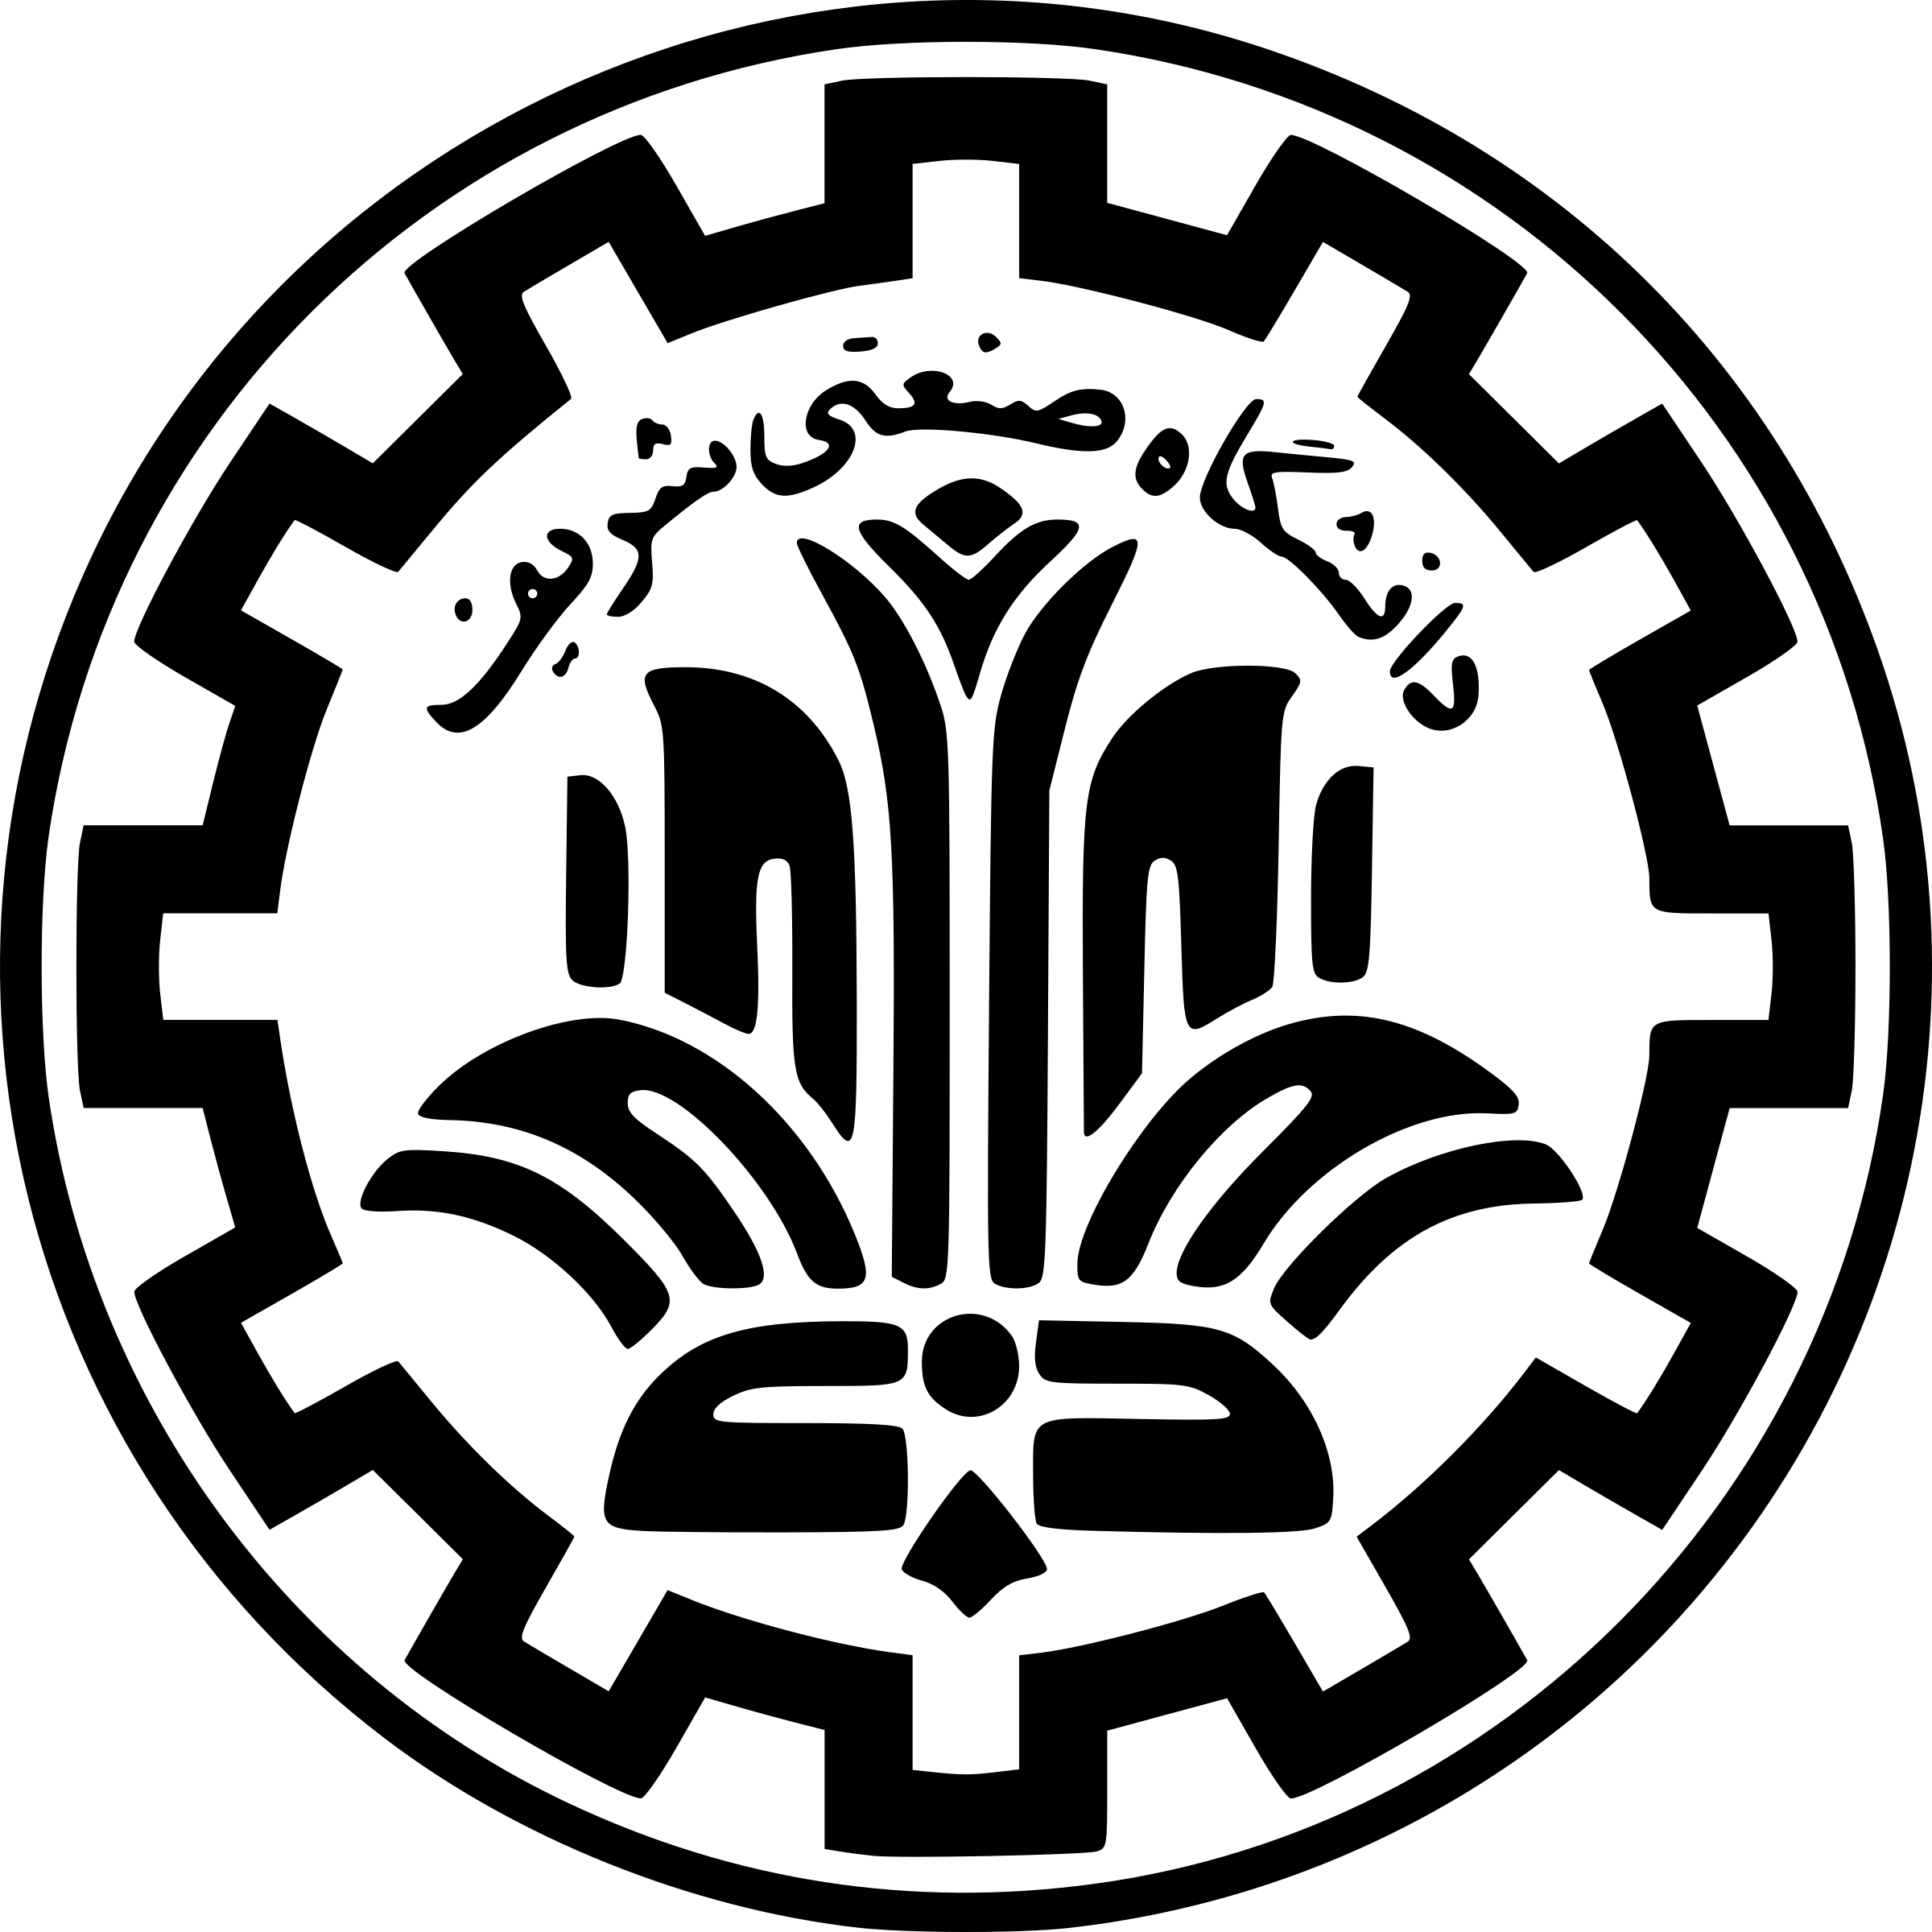
\includegraphics[width=4cm]{sharif.png}\\[1.5cm]
		{\Large\textbf{دانشگاه صنعتی شریف}}\\[0.5cm]
		{\large\textbf{دانشکده‌ی مهندسی کامپیوتر}}\\[1.5cm]
		{\Huge\textbf{گزارش کار آزمایشگاه}}\\[0.5cm]
		{\LARGE\textbf{آزمایشگاه سیستم‌های عامل}}\\[2cm]
		
		\textbf{گزارش آزمایش شماره ۲}\\
		(آشنایی با فراخوانی‌های سیستمی)
		
		\vfill
		\begin{tabular}{rl}
			\textbf{شماره‌ی گروه:} & ۲۰ \\
			\textbf{گروه:} &
			ارشیا یوسف‌نیا (۴۰۱۱۱۰۴۱۵) \\
			& محمدعارف زارع زاده (۴۰۱۱۰۶۰۱۷) \\
			\textbf{استاد درس:} & دکتر بیگی \\
			\textbf{تاریخ:} & تابستان ۱۴۰۴ \\
		\end{tabular}
	\end{titlepage}
	
	% ==============================
	% Persian Ordinal Page Numbering
	% ==============================
	\clearpage
	\setcounter{page}{1}
	\renewcommand{\thepage}{\persianordinalpage}
	
	\tableofcontents
	\clearpage
	\listoffigures
	\clearpage
	\listoftables
	
	% ==============================
	% Switch to Persian Digits (۱, ۲, ۳, ...)
	% ==============================
	\clearpage
	\setcounter{page}{1}
	\pagenumbering{arabic}
	\renewcommand{\thepage}{\persianfont\arabic{page}}
	
	
	% ==============================
	% Main Content
	% ==============================
        \section{شرح آزمایش}
        \subsection{مشاهده‌ی فراخوانی‌های سیستمی تعریف شده}
        مانند شکل 
        \ref{im1}
        فایل گفته شده را باز کرده و محتویات آن را در شکل
        \ref{im2}
        می‌توان مشاهده کرد. همانطور که می‌توان مشاهده کرد، به ازای هر فراخوانی سیستم، یک ماکرو به فرمت
        \textenglish{\_\_NR\_[syscall name]}
        وجود دارد تا نیاز نباشد هنگام برنامه‌نویسی با آنها، عدد هر فراخوانی سیستم را حفظ کنیم.

        \begin{figure}[H]
		\centering
		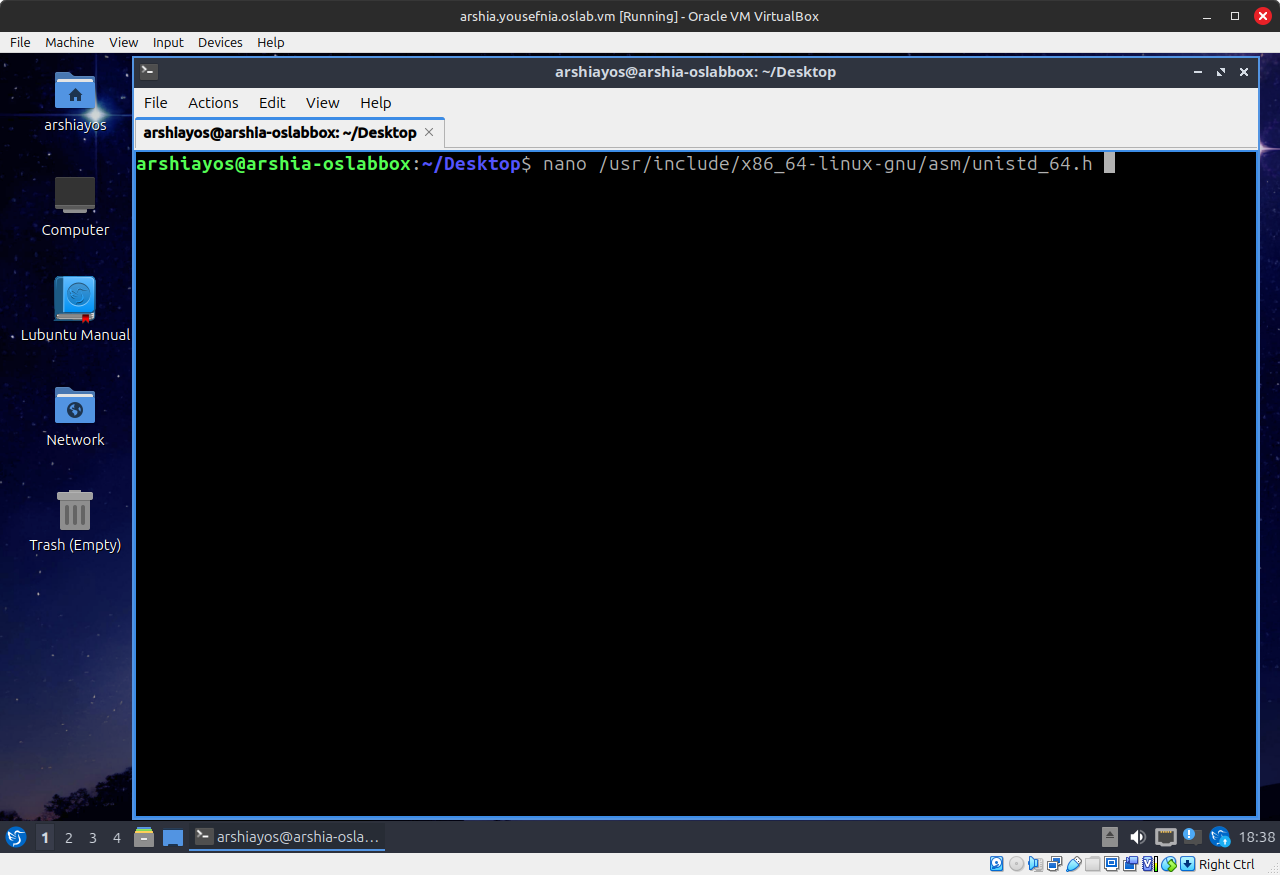
\includegraphics[width=0.8\textwidth]{report2-resources/1.png}
		\caption{خواندن فایل \textenglish{unistd\_64.h}}
            \label{im1}
	\end{figure}

        \begin{figure}[H]
		\centering
		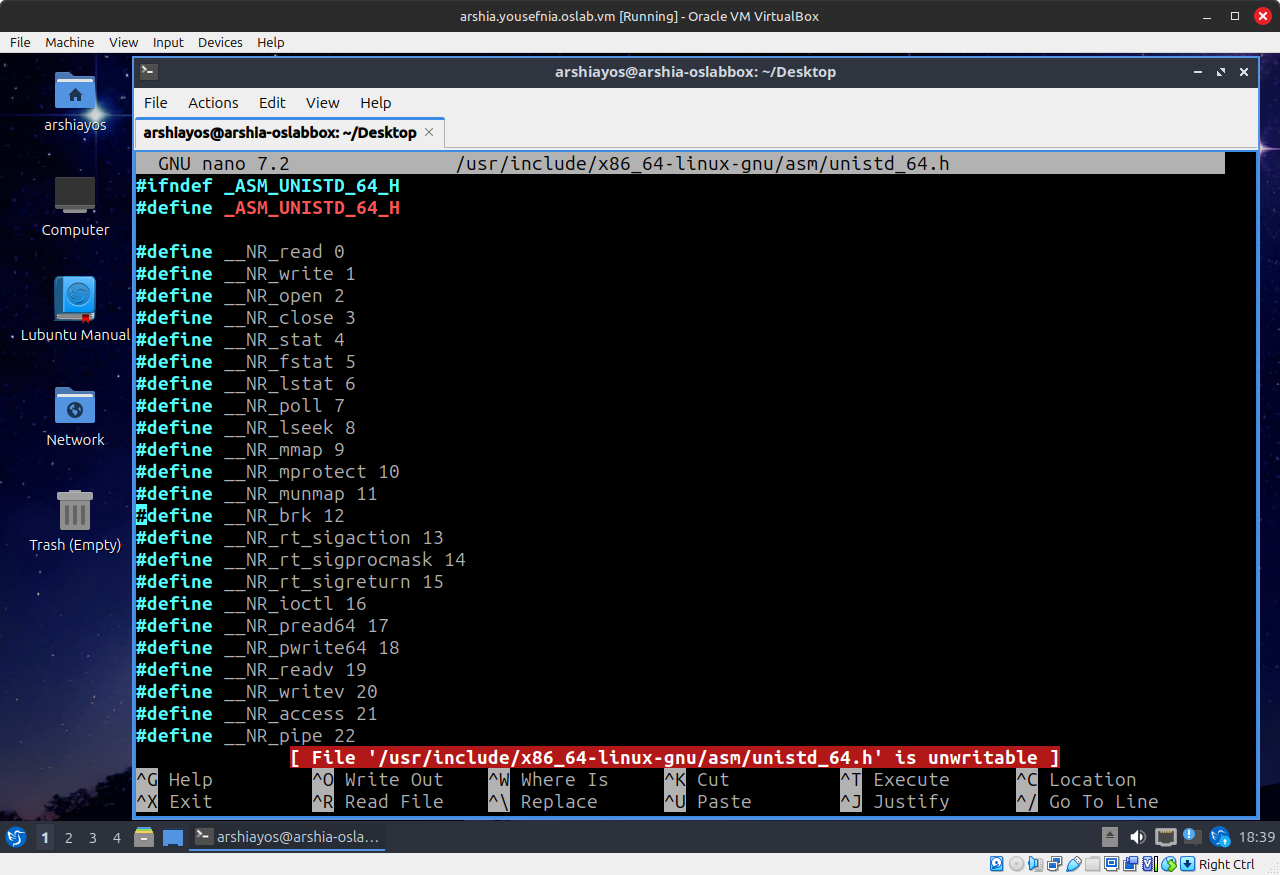
\includegraphics[width=0.8\textwidth]{report2-resources/2.png}
		\caption{محتویات فایل \textenglish{unistd\_64.h}}
            \label{im2}
	\end{figure}

        \subsection{اجرای یک فراخوانی سیستمی}
        \begin{enumerate}
        \item 
        همانطور که از شکل 
        \ref{im3}
        می‌توان دید، فایل را ساخته و کد گفته شده را در ان می‌گذاریم.

        \begin{figure}[H]
		\centering
		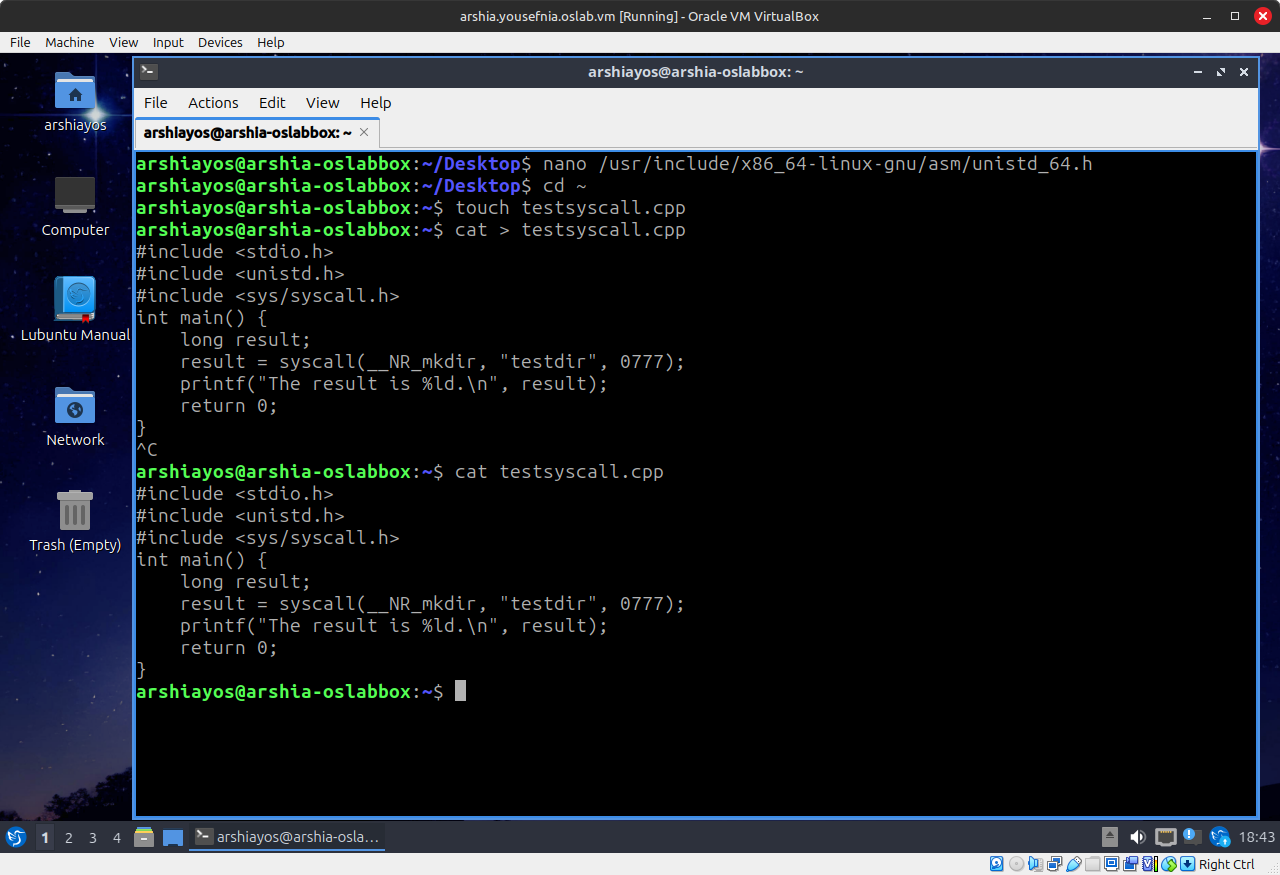
\includegraphics[width=0.8\textwidth]{report2-resources/3.png}
		\caption{کد ساخت پوشه با استفاده از فراخوانی سیستمی}
        \label{im3}
	\end{figure}

        

        \item کد را در شکل
        \ref{im3}
        می‌توان دید.

        \item خروجی حاصل از اجرای این کد را در شکل زیر می‌توان مشاهده کرد.

        \begin{figure}[H]
		\centering
		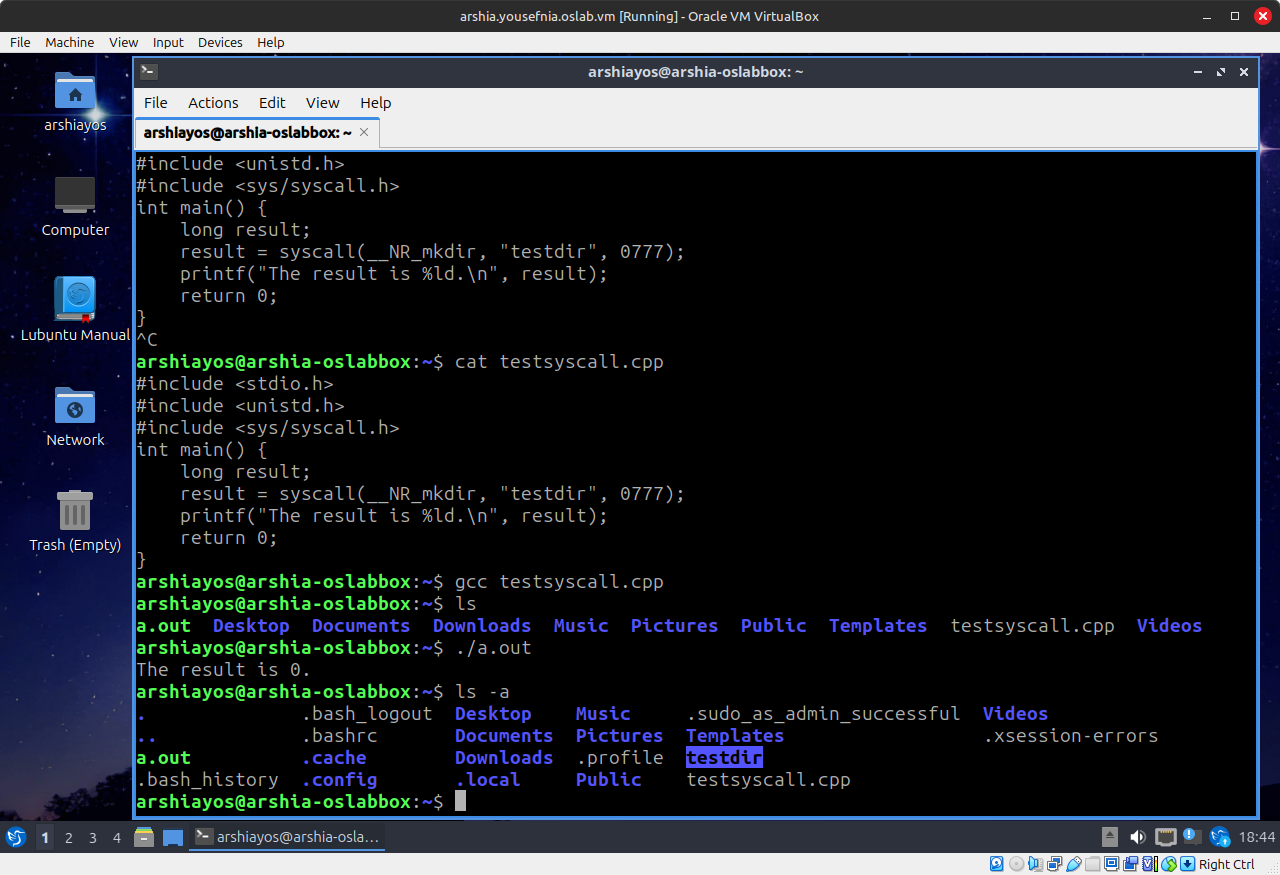
\includegraphics[width=0.8\textwidth]{report2-resources/5.png}
		\caption{ساخت پوشه با استفاده از فراخوانی سیستمی}
	\end{figure}

        \item این کد ابتدا با دستور 
        syscall
        و با کمک شماره‌ی فراخوانی سیستمی 
        mkdir
        آن را اجرا می‌کند.
        تابع
        syscall 
        در آرگومان اول خود شماره‌ی فراخوانی سیستمی و در آرگومان‌های بعدی خود، آرگومان‌هایی که به آن فراخوانی سیستمی داده می‌شود را می‌دهیم.

        آرگومان 
        testdir
        نام پوشه‌ای که ساخته می‌شود است، و عدد
        0777
        که در مبنای 8 است، سطوح دسترسی را مشخص می‌کند، که در این نمونه، همه دسترسی خواندن و نوشتن و اجرا کردن را دارند.

        سپس خروجی 
        syscall
        در متغیر 
        result
        ریخته می‌شود. به طور کلی هنگام فراخوانی‌های سیستمی، خروجی اگر 0 باشد یعنی مشکلی نبوده و اگر 
        \textenglish{-1}
        باشد، یعنی به خطا خورده است.

        درنهایت این خروجی چاپ شده و برنامه تمام می‌شود.

        درستی کارکرد آن را نیز در شکل بالا می‌توان دید.

        پاسخ به تمرین‌های این بخش:

        \begin{enumerate}
            \item نقش 
            \textenglish{\_\_NR\_mkdir}
            که یک ماکرو است، دادن شماره‌ی فراخوانی سیستمی
            mkdir
            به تابع
            syscall
            است. آن را در شکل
            \ref{im2}
            نیز می‌توان مشاهده کرد.

            \item همانطور که در بالا نیز توضیح داده شد، آرگومان اول تابع
            syscall
            شماره‌ی فراخوانی سیستمی است، و آرگومان‌های بعدی، ورودی‌ها یا آرگومان‌های مربوط به آن فراخوانی سیستم (برای اجرا کردن) است.

            خروجی تابع
            syscall
            هم عموما یا \textenglish{0} و یا 
            \textenglish{-1}
            است.
            اگر \textenglish{0} باشد یعنی فراخوانی سیستمی بدون هیچ مشکلی اجرا شده و عملیات آن موفق بوده، و اگر
            \textenglish{-1}
            باشد یعنی فراخوانی سیستمی به خطا خورده، و همچنین
            \textenglish{errno}
            با توجه به شماره‌ی خطای خورده شده را می‌گیرد.
        \end{enumerate}
        
        \end{enumerate}

        \subsection{اجرای ساده‌تر فراخوانی سیستمی}
        کد مربوط به
        \textenglish{testsyscall2.cpp}
        را در شکل زیر می‌توانید مشاهده کنید.
        این کد با کد بخش قبل تقریبا هیچ تفاوتی ندارد. تنها تفاوت آن این است که به جای استفاده از تابع
        \textenglish{syscall}
        از تابع
        \textenglish{mkdir}
        استفاده شده است. ورودی‌های آن هم به جز ورودی اول (که به وضوح دیگر لازم نیست) مانند ورودی‌های تابع
        \textenglish{syscall}
        است.

        \begin{figure}[H]
		\centering
		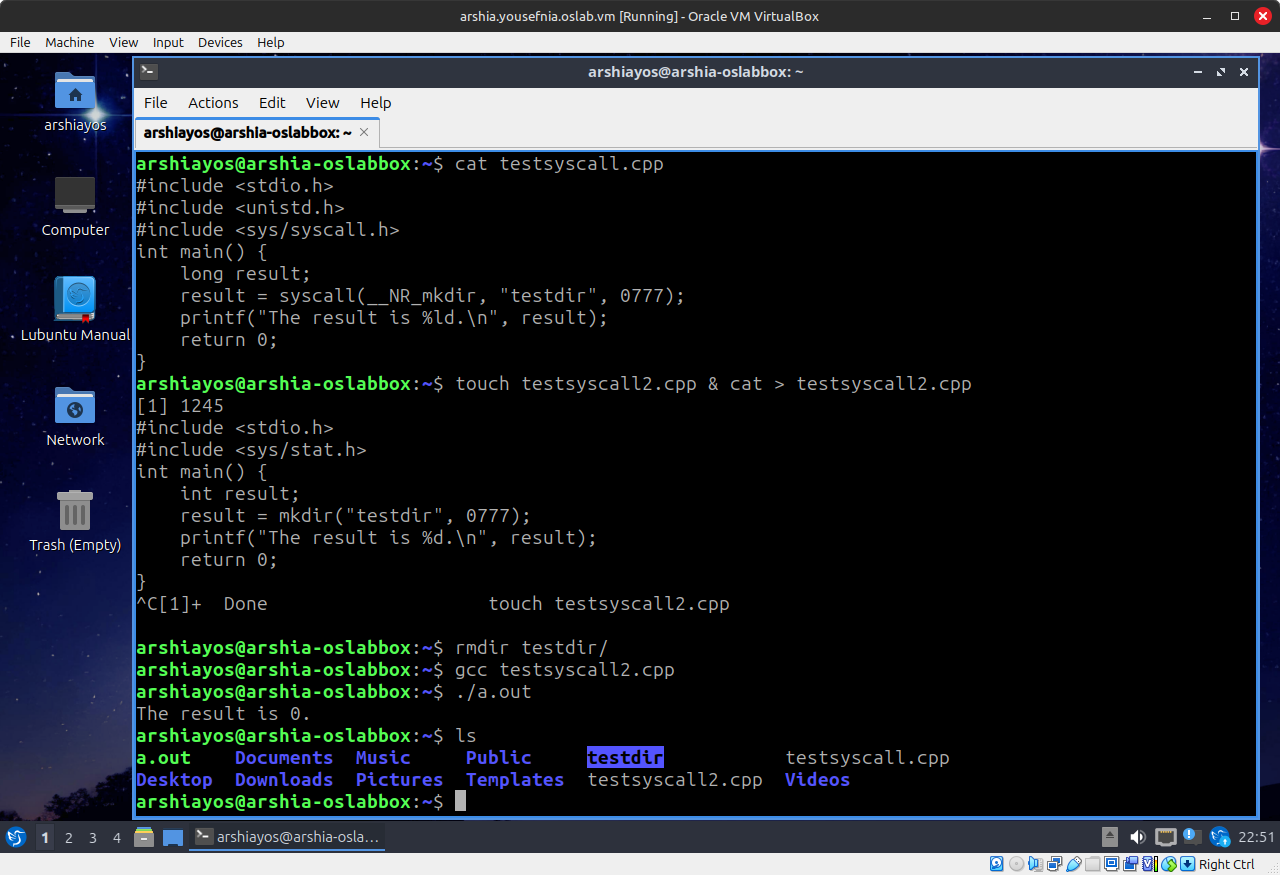
\includegraphics[width=0.8\textwidth]{report2-resources/6.png}
		\caption{استفاده از تابع \textenglish{mkdir} به جای \textenglish{syscall}}
	\end{figure}


        \subsection{آشنایی با چند فراخوانی سیستمی پرکاربرد}
        \begin{itemize}
        \item 
        
        
        فراخوانی سیستمی 
        \textenglish{access}
        دو آرگومان ورودی دارد: اولی نام/آدرس فایل و دومی 
        \textenglish{Mode}
        است. مدهای مختلف آن را در جدول زیر می‌توانید مشاهده کنید
        \cite{linux-man-access}
        . برای اینکه چند مد مختلف با هم تست شوند، می‌توان مدهای مورد نظر را با هم 
        \textenglish{or}
        محاسباتی (نه منطقی)
        کرد.

        \begin{table}[h!]
            \centering
            \begin{tabular}{|c|c|}
            \hline
            \textenglish{}{Mode} & توضیحات \\
            \hline
            \textenglish{F\_OK} & بررسی اینکه فایل وجود دارد \\
            \hline
            \textenglish{R\_OK} & بررسی اینکه فایل قابل خواندن است \\
            \hline
            \textenglish{W\_OK} & بررسی اینکه فایل قابل نوشتن است \\
            \hline
            \textenglish{X\_OK} & بررسی اینکه فایل قابل اجرا کردن است. \\
            \hline
            \end{tabular}
            \caption{\textenglish{Mode}های مختلف برای فراخوانی سیستمی \textenglish{access}}
        \end{table}

        طبق این توضیحات، در شکل زیر می‌توانید کد مورد نظر را مشاهده کنید. در این کد ابتدا چک می‌شود که تعداد آرگومان‌ها درست باشد، سپس به ترتیب وجود داشتن،‌ دسترسی خواندن، و دسترسی نوشتن چک می‌شود.

        \begin{figure}[H]
		\centering
		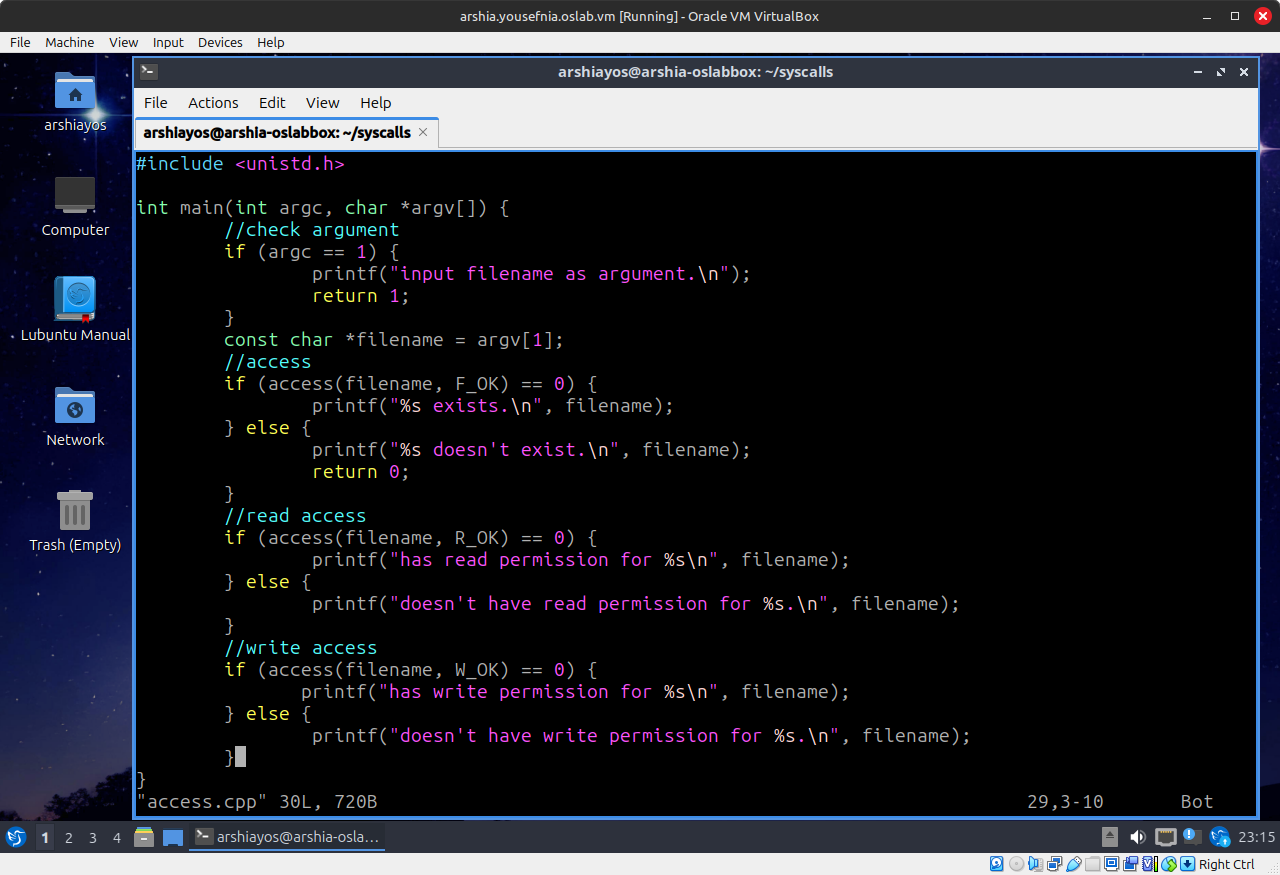
\includegraphics[width=0.8\textwidth]{report2-resources/7.png}
		\caption{کد برنامه‌ی بررسی فایل و سطوح دسترسی برای پردازه‌ی اجرا شده}
	\end{figure}

        \begin{figure}[H]
		\centering
		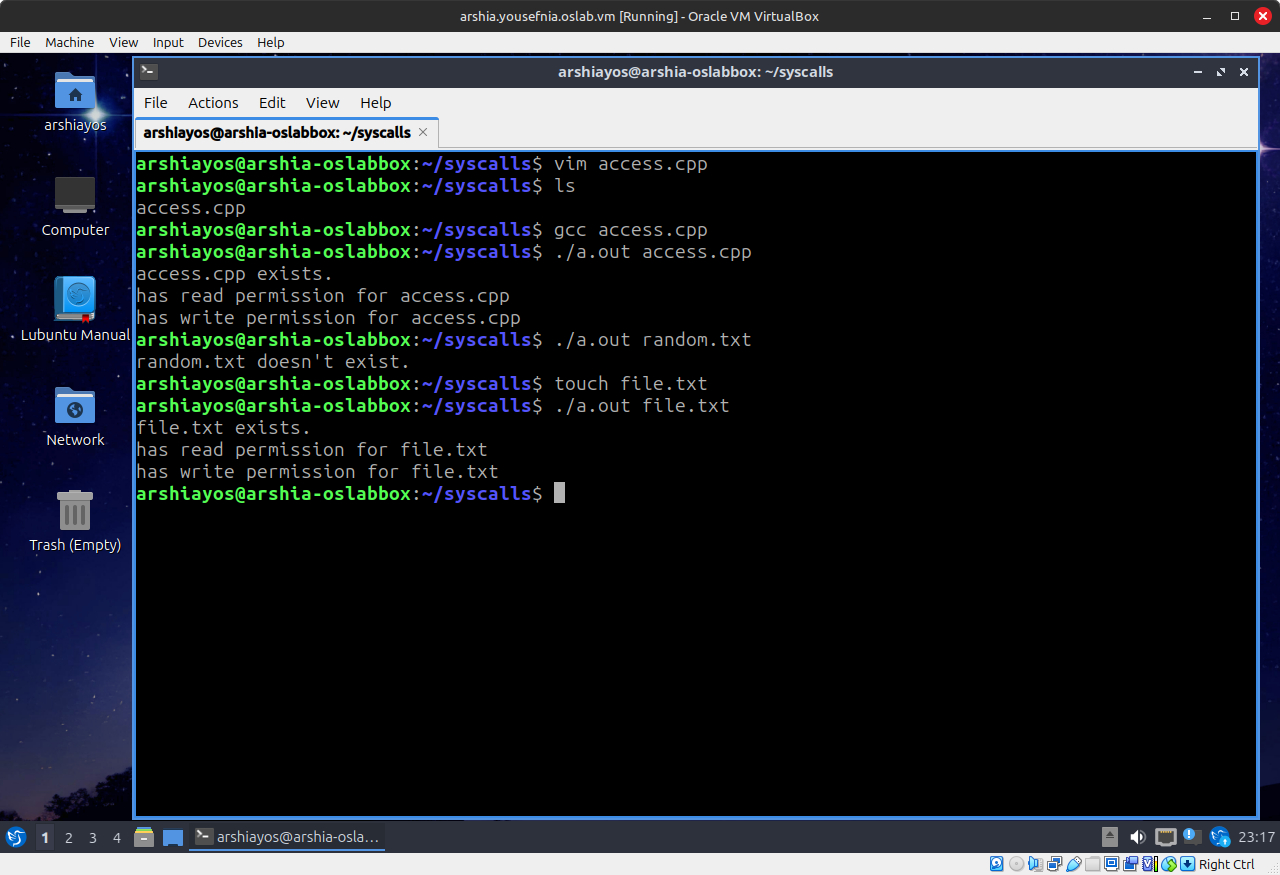
\includegraphics[width=0.8\textwidth]{report2-resources/8.png}
		\caption{اجرای کد بالا}
	\end{figure}

        \item
        فراخوانی سیستمی 
        \textenglish{open}
        سه آرگومان را به عنوان ورودی می‌گیرد. اولی نام فایلی که می‌خواهیم باز کنیم است. دومی فلگ‌های مربوط به آن است. سومی هم سطوح دسترسی، در صورت استفاده از فلگ
        \textenglish{O\_CREAT}
        است. انواع فلگ‌ها را در تصویر زیر می‌توانید مشاهده کنید
        \cite{linux-man-open}
        . برای استفاده از چندین فلگ می‌توان آنها را با هم
        \textenglish{or}
        کرد.

        \begin{table}[h!]
            \centering
            \begin{tabular}{|c|c|}
            \hline
            \textenglish{}{Flag} & توضیحات \\
            \hline
            \textenglish{}{O\_RDONLY} & برای باز کردن و فقط خواندن \\
            \hline
            \textenglish{}{O\_WRONLY} & برای باز کردن و فقط نوشتن \\
            \hline
            \textenglish{}{O\_RDWR} & برای باز کردن و خواندن و نوشتن \\
            \hline
            \textenglish{}{O\_CREAT} & برای ساخت فایل درصورت وجود نداشتن (نیاز به آرگومان سطح دسترسی دارد) \\
            \hline
            \textenglish{}{O\_EXCL} & همراه با \textenglish{O\_CREAT} درصورت وجود داشتن فایل از قبل، خطا بخورد\\
            \hline
            \textenglish{}{O\_APPEND} & با هربار نوشتن، داده به انتهای فایل اضافه شود \\
            \hline
            \textenglish{}{O\_TRUNC} & درصورت وجود فایل، محتویات آن خالی شود \\
            \hline
            \textenglish{}{O\_NONBLOCK} &  باز کردن در  حالت \textenglish{non-blocking}\\
            \hline
            \textenglish{}{O\_SYNC} & نوشتن به صورت هماهنگ (سنکرون) باشد. \\
            \hline
            \end{tabular}
            \caption{فلگ‌های فراخوانی سیستمی \textenglish{open}}
        \end{table}

        خروجی 
        \textenglish{open}
        درصورت موفق بودن عملیات 
        عددی مثبت که بیانگر
        \textenglish{file decriptor}
        است خواهد بود، و در غیر این صورت
        \textenglish{-1}
        خواهد بود.

        فراخوانی سیستمی
        \textenglish{write}
        سه آرگومان دارد. اولی 
        \textenglish{file decriptor}
        که همان خروجی
        \textenglish{open}
        است، دومی یک پوینتر به چیزی که می‌خواهیم بنویسیم، و سومی تعداد بایت‌هایی که می‌خواهیم بنویسیم است 
        \cite{linux-man-write}
        .

        خروجی آن درصورت موفق بودن، تعداد بایت‌هایی که نوشته‌ شده‌اند است، و در صورت خطا خوردن 
        \textenglish{-1}
        است.

        فراخوانی سیستمی 
        \textenglish{close}
        فقط یک آرگومان ورودی دارد که همان
        \textenglish{file decriptor}
        است. خروجی آن هم در صورت موفق بودن 
        \textenglish{0}
        و در غیر این صورت
        \textenglish{-1}
        است
        \cite{linux-man-close}
        .

        کد مربوط به خواسته‌ی این بخش را در شکل زیر می‌توانید ببینید. این کد ابتدا با 
        \textenglish{open}
        با کمک فلگ‌های مناسب
        فایل را درصورت وجود نداشتن ساخته و در صورت وجود داشتن آن را خالی کرده و آن را در حالت فقط نوشتن باز می‌کند. سپس با دستور
        \textenglish{write}
        محتویات خواسته شده را (که 17 بایت است) را در آن فایل می‌نویسد. درنهایت آن را با دستور
        \textenglish{close}
        می‌بندد. در صورت خطا داشتن در هر یک از مراحل، خطای مناسبی را چاپ کرده و خارج می‌شوند.

        \begin{figure}[H]
		\centering
		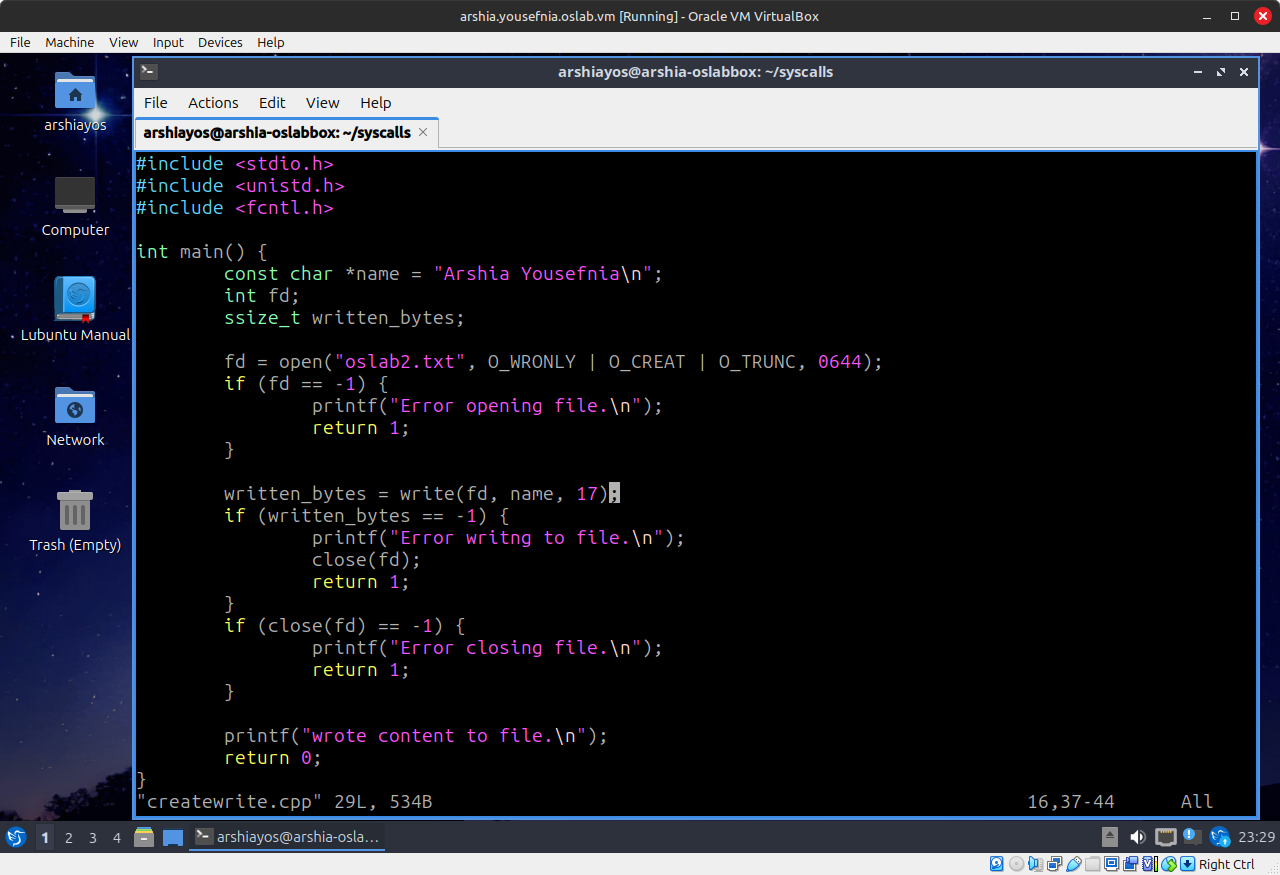
\includegraphics[width=0.8\textwidth]{report2-resources/9.png}
		\caption{کد ساخت و نوشتن اسم در فایل}
	\end{figure}

        \begin{figure}[H]
		\centering
		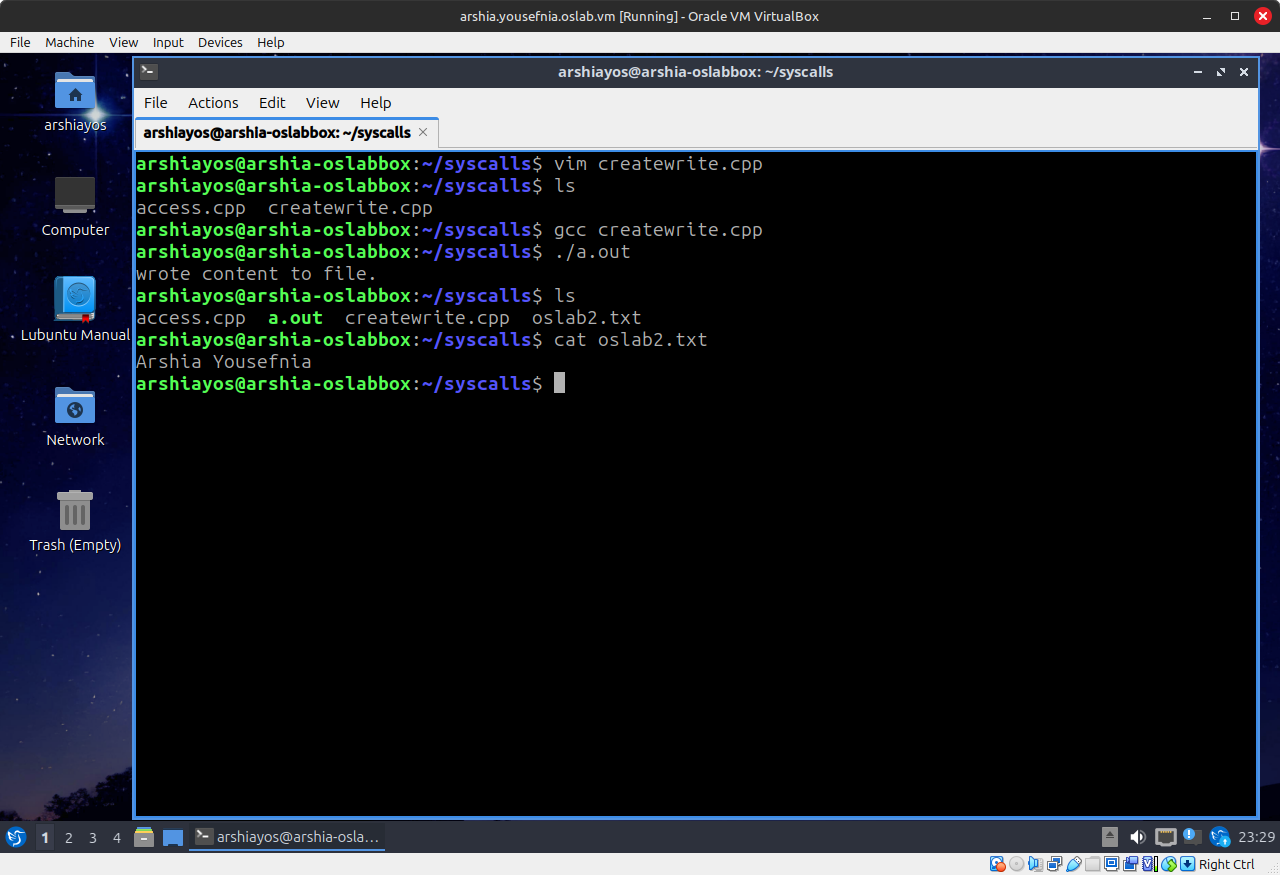
\includegraphics[width=0.8\textwidth]{report2-resources/10.png}
		\caption{اجرای کد بالا}
	\end{figure}
        
        \item 
        فراخوانی سیستمی 
        \textenglish{sysinfo}
        فقط یک آرگومان که از نوع پوینتر به
        \textenglish{struct sysinfo}
        است را ورودی گرفته و خروجی‌اش درصورت موفق بودن 
        \textenglish{0}
        و در غیر این صورت
        \textenglish{-1}
        است.

        همچنین پس از اجرای موفقیت آمیز آن، 
        \textenglish{struct sysinfo}
        که ورودی فراخوانی سیستم به آن اشاره می‌کرد، براساس اطلاعات سیستم پر می‌شود.

        در
        \textenglish{struct sysinfo}
        فیلدهای زیادی درمورد اطلاعات سیستم وجود دارد، اما دو موردی که ما به آن نیاز داریم، 
        \textenglish{totalram}
        و 
        \textenglish{freeram}
        که به ترتیب کل حافظه 
        \textenglish{RAM}
        و حافظه‌ی خالی است می‌باشند
        \cite{linux-man-sysinfo}
        .

        در شکل زیر کد مربوط به خواسته‌ی این بخش را می‌توان مشاهده کرد. این کد ابتدا فراخوانی سیستمی را انجام می‌دهد، سپس درصورت خطا داشتن، پیغام خطا چاپ می‌کند و درصورت خطا نداشتن، اطلاعات خواسته شده را چاپ می‌کند.

        \begin{figure}[H]
		\centering
		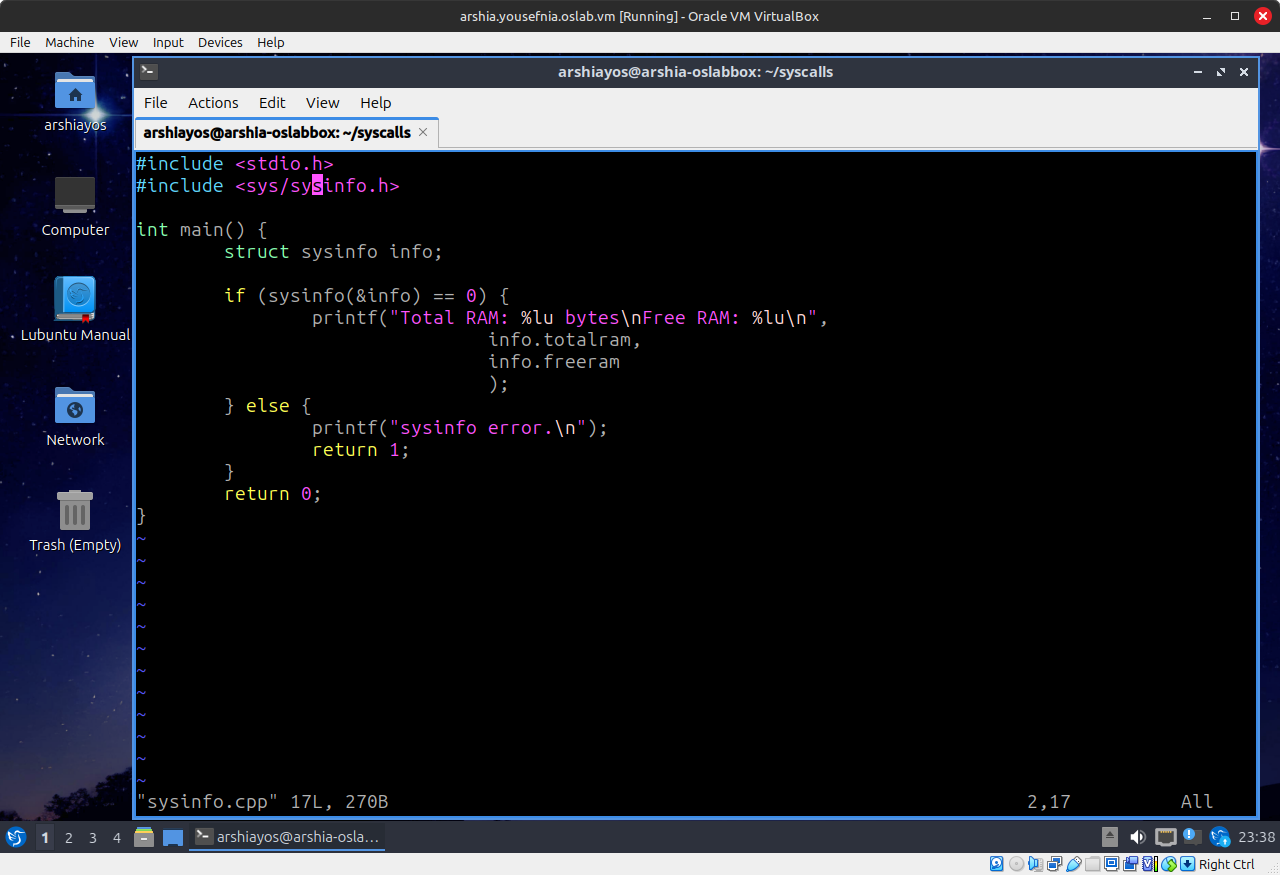
\includegraphics[width=0.8\textwidth]{report2-resources/11.png}
		\caption{کد برنامه‌ی چاپ اطلاعات رم}
	\end{figure}

        \begin{figure}[H]
		\centering
		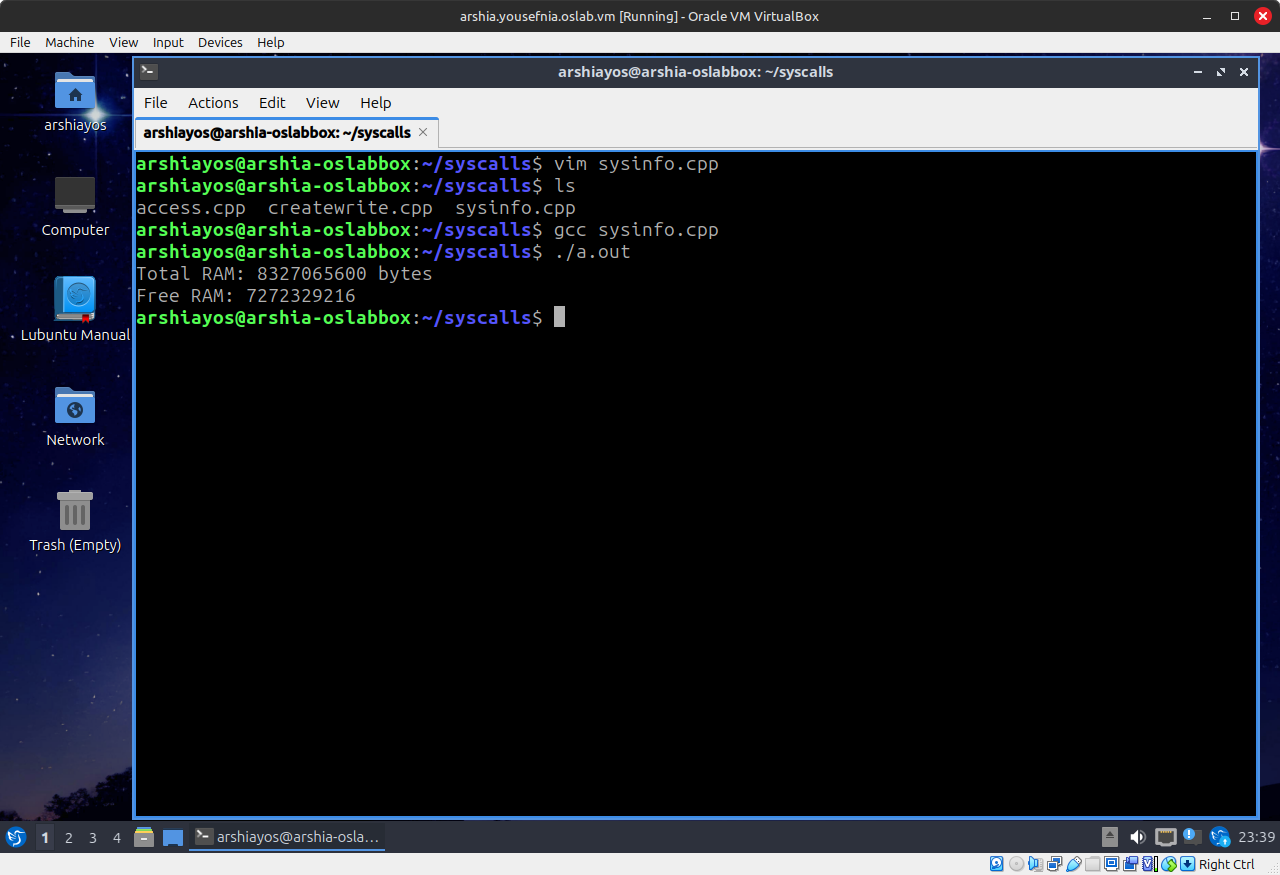
\includegraphics[width=0.8\textwidth]{report2-resources/12.png}
		\caption{اجرای برنامه‌ی چاپ اطلاعات رم}
	\end{figure}

        \item 
        فراخوانی سیستمی
        \textenglish{getrusage}
        دو آرگومان به عنوان ورودی می‌گیرد. اولی مشخص می‌کند که اطلاعات مصرف حافظه برای چه پردازه‌ها یا ترد‌هایی محاسبه شود. از مقادیر پرکارد آن می‌توان
        \textenglish{RUSAGE\_SELF}
        که به پردازه‌ی اجرا کننده‌ی این فراخوانی سیستمی اشاره می‌کند، 
        \textenglish{RUSAGE\_CHILDREN}
        که به پردازه‌های فرزند این پردازه که اجرایشان تمام شده و در حالت
        \textenglish{wait()}
        هستند اشاره می‌کند، و 
        \textenglish{RUSAGE\_THREAD}
        که به تردی که این دستور را اجرا کرده اشاره می‌کند را بیان کرد
        \cite{linux-man-getrusage}
        .

        آرگومان ورودی دوم هم یک پوینتر به یک
        \textenglish{struct rusage}
        است که قرار است پس از اجرای این فراخوانی سیستمی، فیلدهای درون آن به درستی پر شوند. 

        این استراکت فیلدهای زیادی دارد، اما تنها موردی که در این بخش به آن نیاز داریم، 
        \textenglish{ru\_maxrss}
        است، که میزان حافظه‌ی مصرفی را نشان می‌دهد.

        کد آن را در زیر می‌توان مشاهده کرد. این کد ابتدا فراخوانی سیستم را اجرا می‌کند و درصورت خطا نداشتن، اطلاعات خواسته شده را چاپ می‌کند.

        \begin{figure}[H]
		\centering
		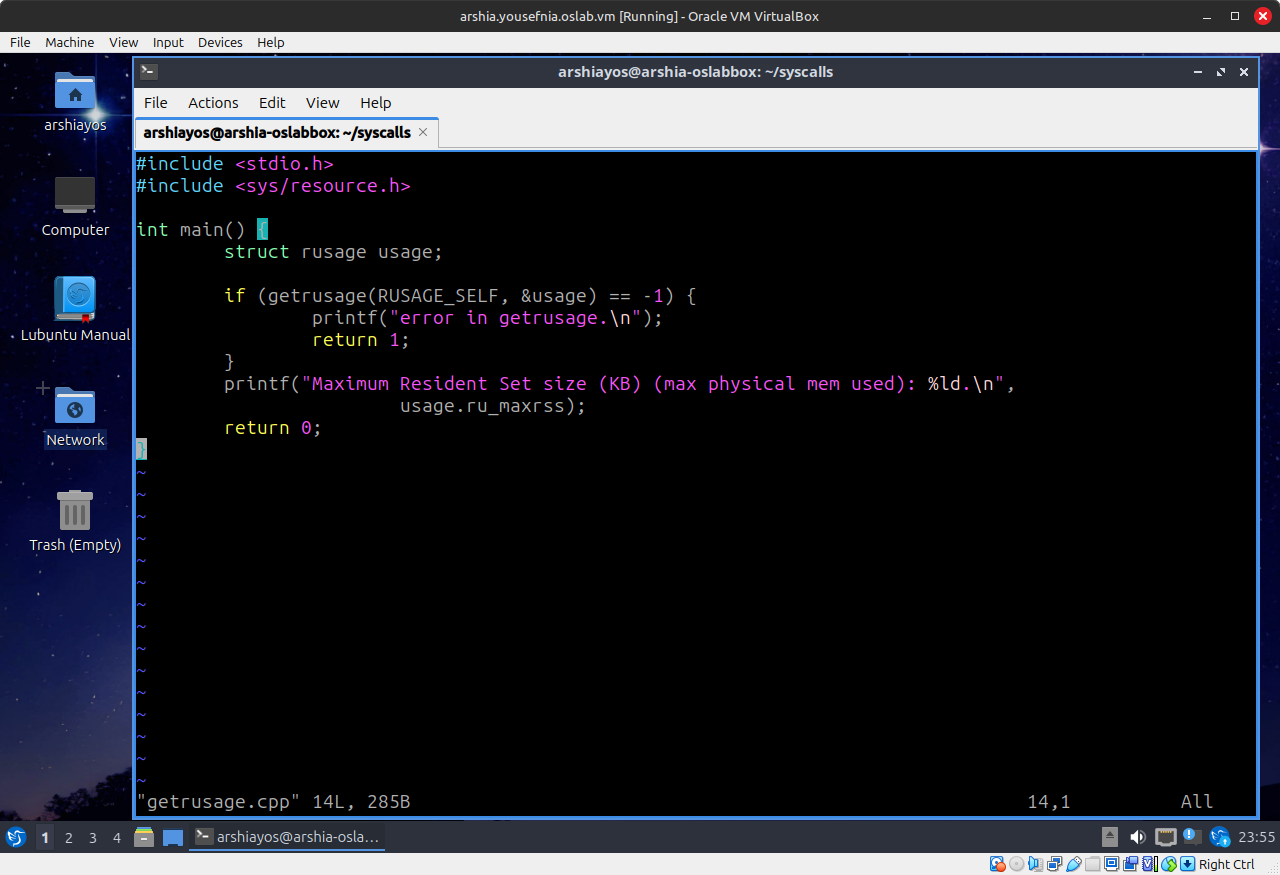
\includegraphics[width=0.8\textwidth]{report2-resources/13.png}
		\caption{کد برنامه‌ی چاپ کننده‌ی حافظه‌ی مصرفی}
	\end{figure}

        \begin{figure}[H]
		\centering
		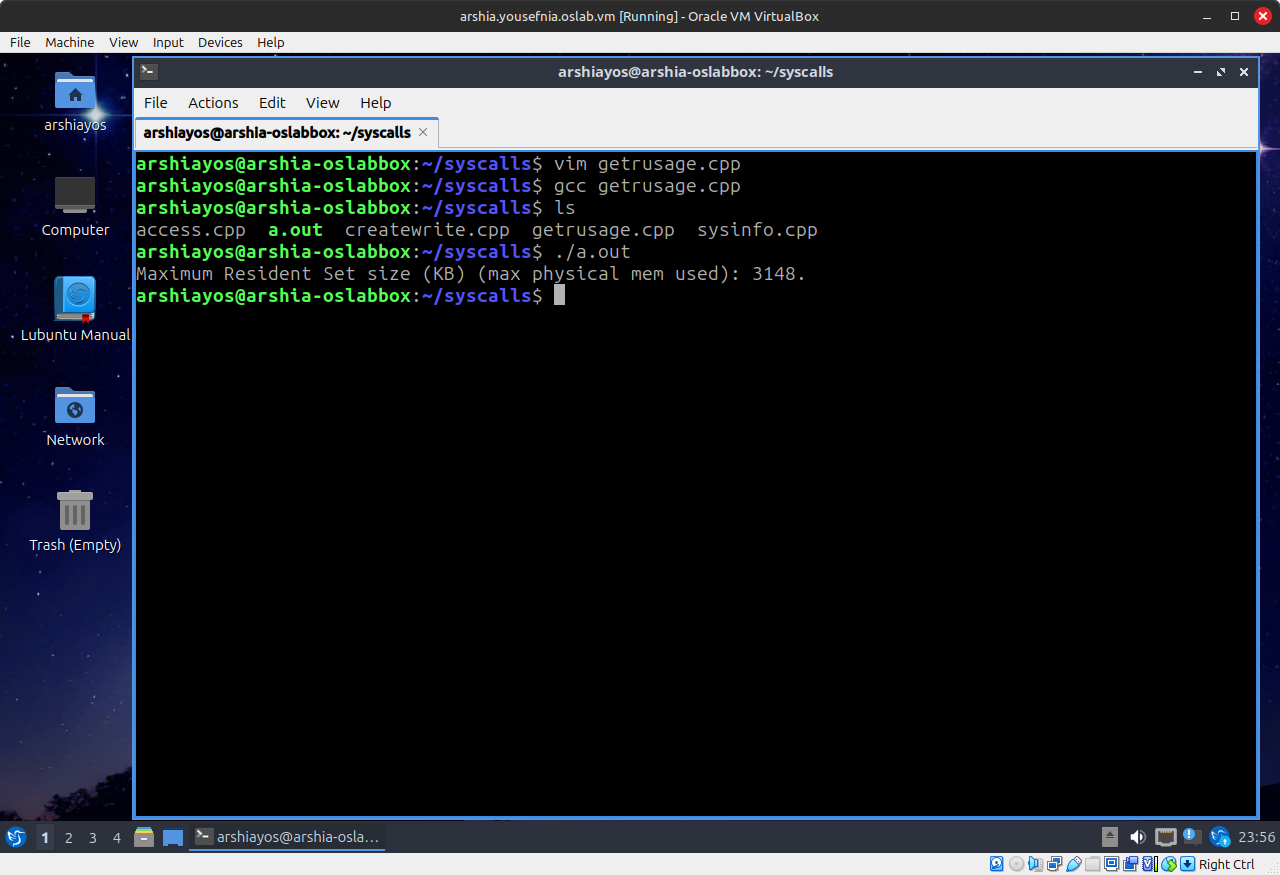
\includegraphics[width=0.8\textwidth]{report2-resources/14.png}
		\caption{اجرای برنامه‌ی چاپ کننده‌ی حافظه‌ی مصرفی}
	\end{figure}
       
        \end{itemize}

        \subsection{اضافه کردن یک فراخوانی سیستمی به سیستم عامل}
        مطابق مراحل دستور کار، هر بخش را توضیح داده و در صورت نیاز، اسکرین شات می‌گذاریم.

        \begin{enumerate}
        \item 
        از آنجایی که فقط یک کاربر داریم و آن کاربر هم دسترسی 
        \textenglish{root}
        دارد، در این مرحله مشکلی نمی‌تواند رخ بدهد.

        \item 
        مطابق شکل زیر، وارد آن شده‌ایم.

        \begin{figure}[H]
		\centering
		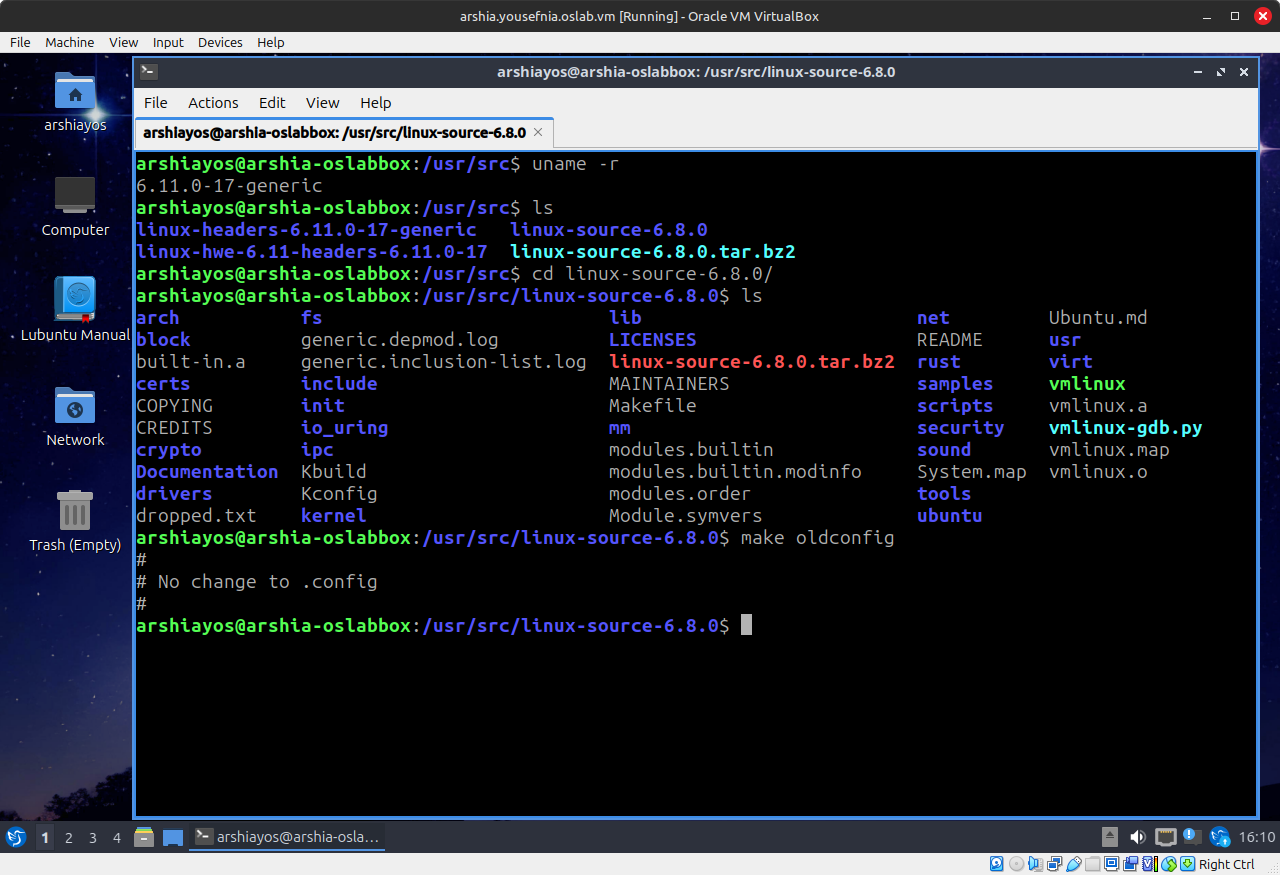
\includegraphics[width=0.8\textwidth]{report2-resources/15.png}
		\caption{ورود به پوشه‌ی کد منبع هسته‌ی سیستم عامل}
            \label{im15}
	\end{figure}

        \item 
        در شکل
        \ref{im15}
        می‌توان خروجی اجرای این دستور را مشاهده کرد.

        \item 
        درستی اجرای این عملیات در شکل زیر قابل مشاهده است.

        \begin{figure}[H]
		\centering
		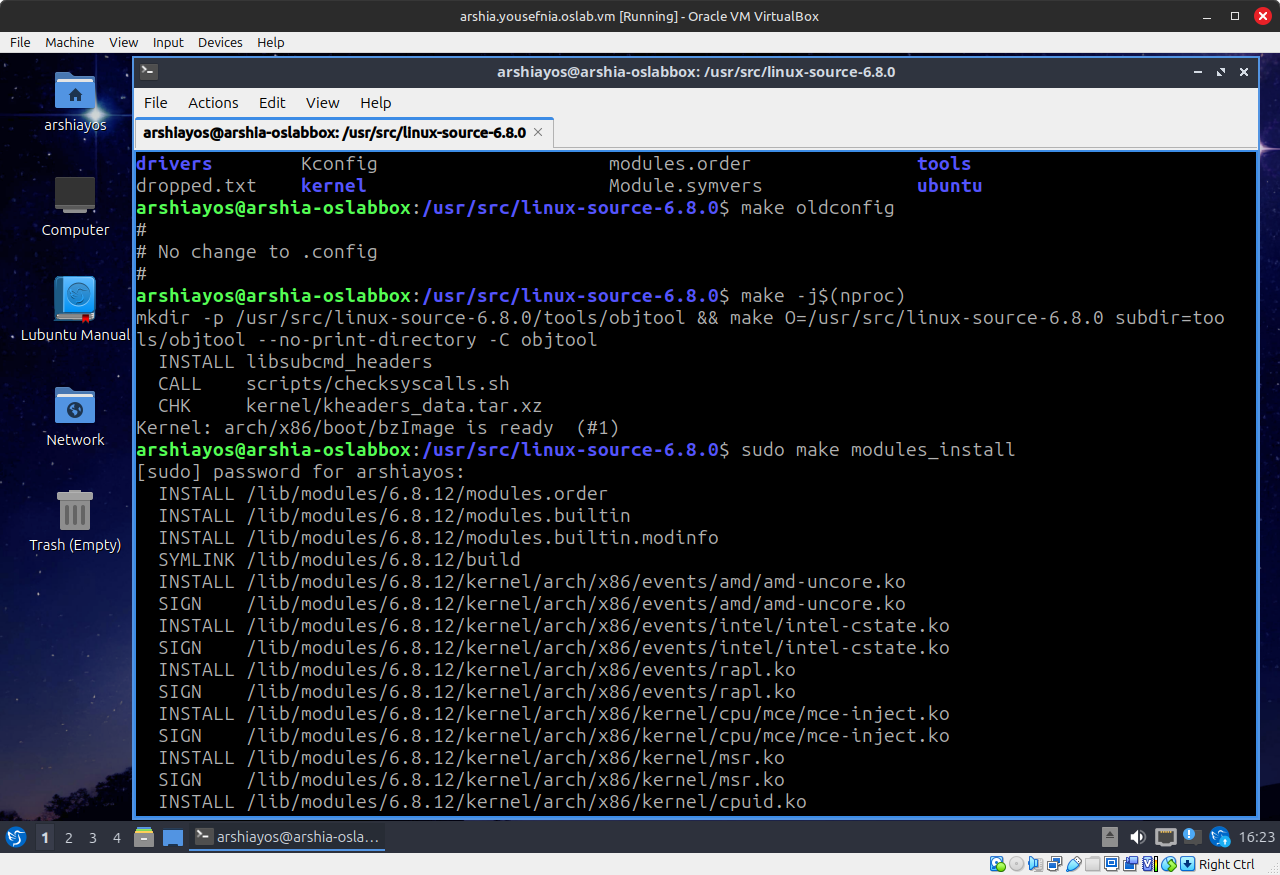
\includegraphics[width=0.8\textwidth]{report2-resources/17.png}
		\caption{درستی کامپایل هسته}
	\end{figure}

        \item 
        نصب هسته‌ی جدید را دوباره انجام می‌دهیم.

        \begin{figure}[H]
		\centering
		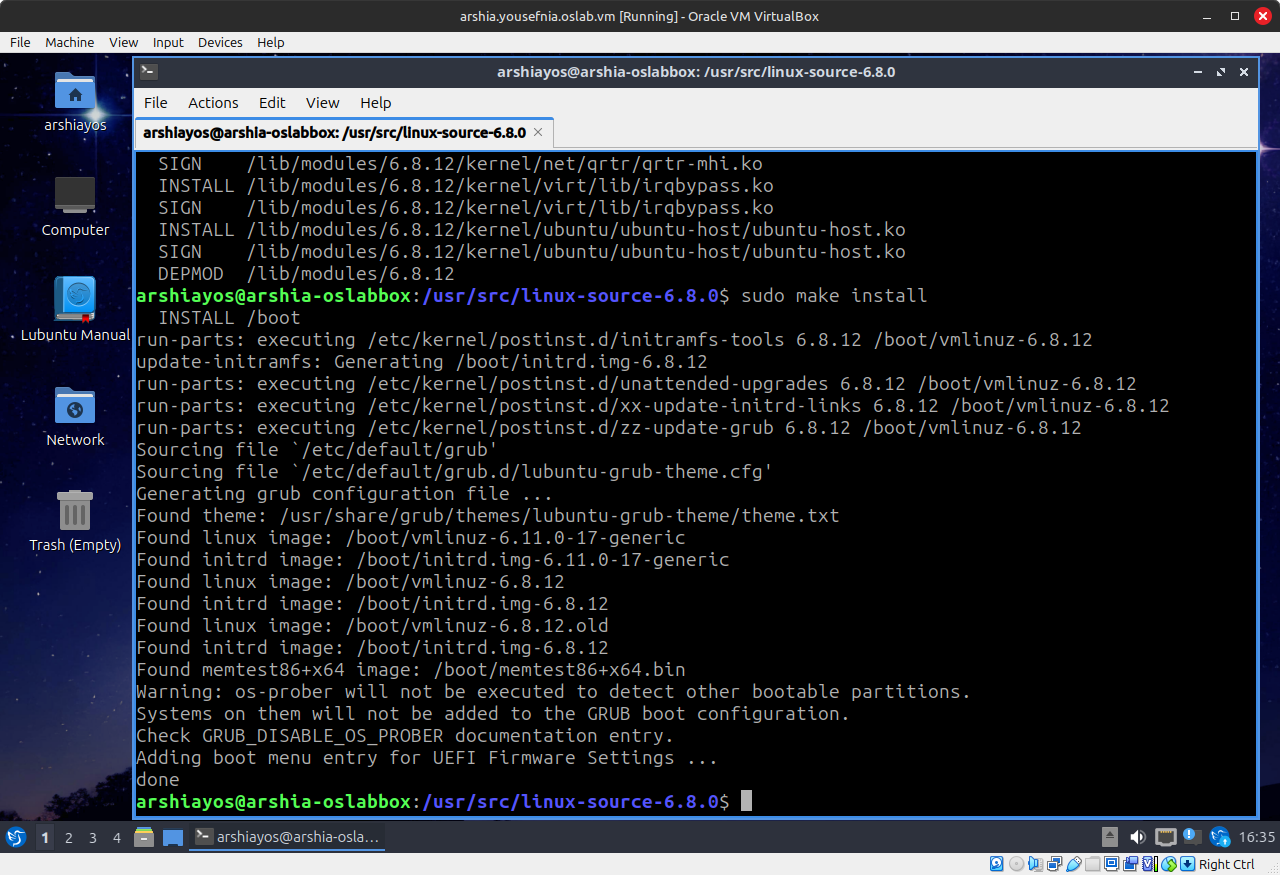
\includegraphics[width=0.8\textwidth]{report2-resources/18.png}
		\caption{نصب هسته‌ی جدید}
	\end{figure}

        \item 
        سیستم را 
        \textenglish{reboot}
        کرده و سیستم عامل را دوباره اجرا می‌کنیم.

        \begin{figure}[H]
		\centering
		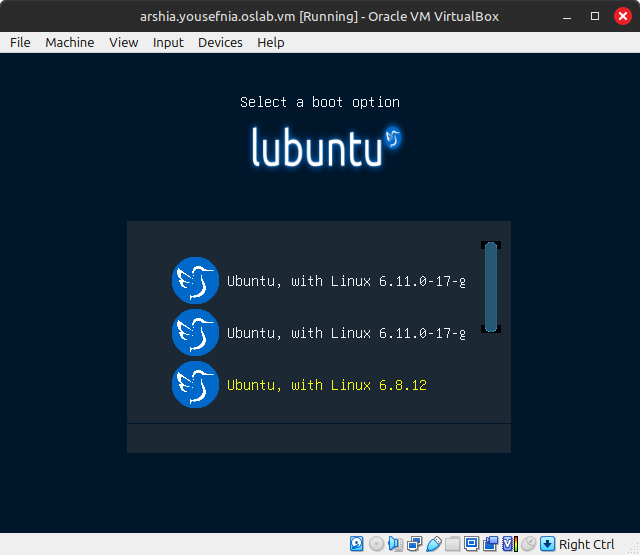
\includegraphics[width=0.8\textwidth]{report2-resources/20.png}
		\caption{\textenglish{reboot} کردن سیستم}
	\end{figure}

        \item 
        مطابق دستور کار، پوشه‌ی 
        \textenglish{hello}
        را می‌سازیم.

        \begin{figure}[H]
		\centering
		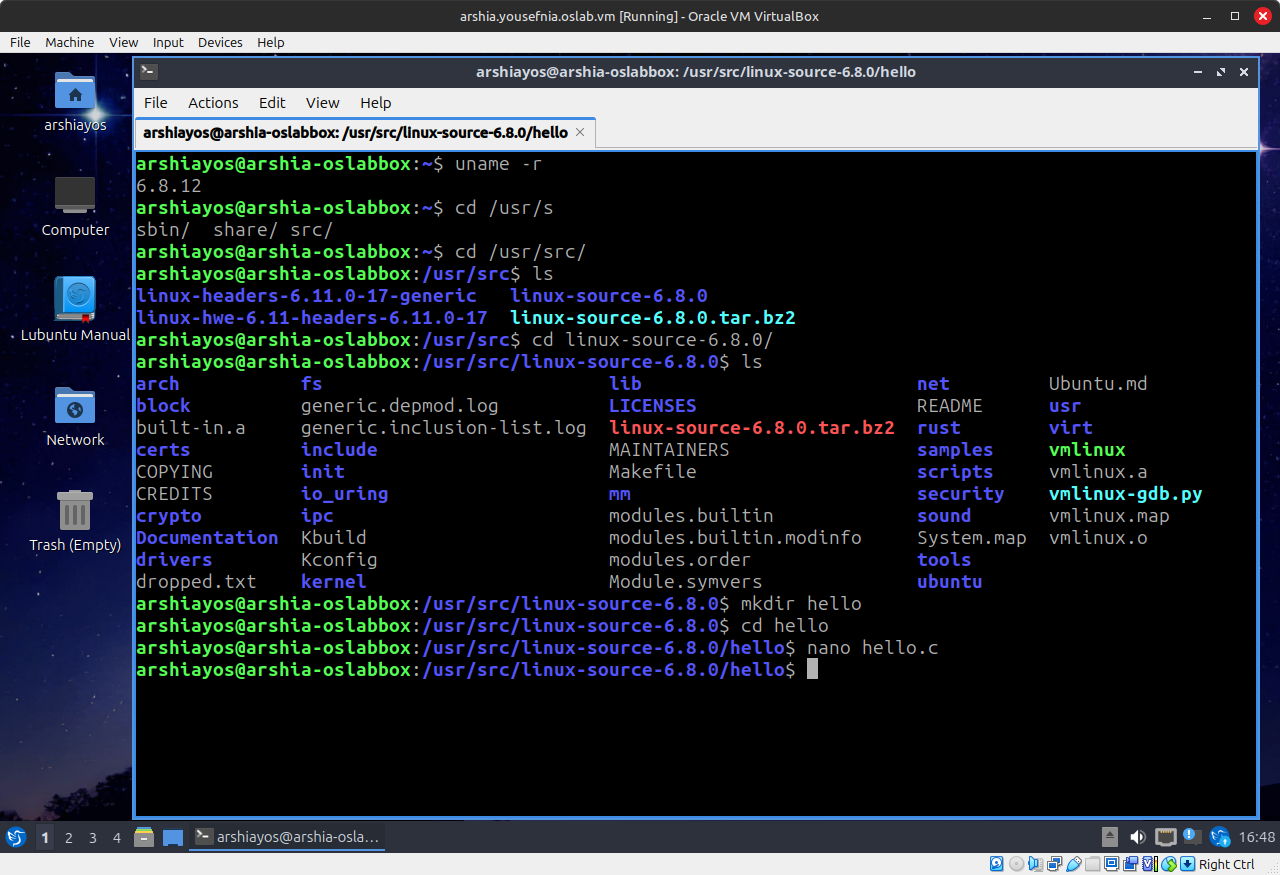
\includegraphics[width=0.8\textwidth]{report2-resources/21.png}
		\caption{ساخت پوشه‌ی \textenglish{hello} و فایل \textenglish{hello.c}}
	\end{figure}

        \item 
        کد داده شده را با کم تغییر (به دلیل ورژن‌های مختلف سیستم عامل) در فایل
        \textenglish{hello.c}
        می‌نویسیم.

        \begin{figure}[H]
		\centering
		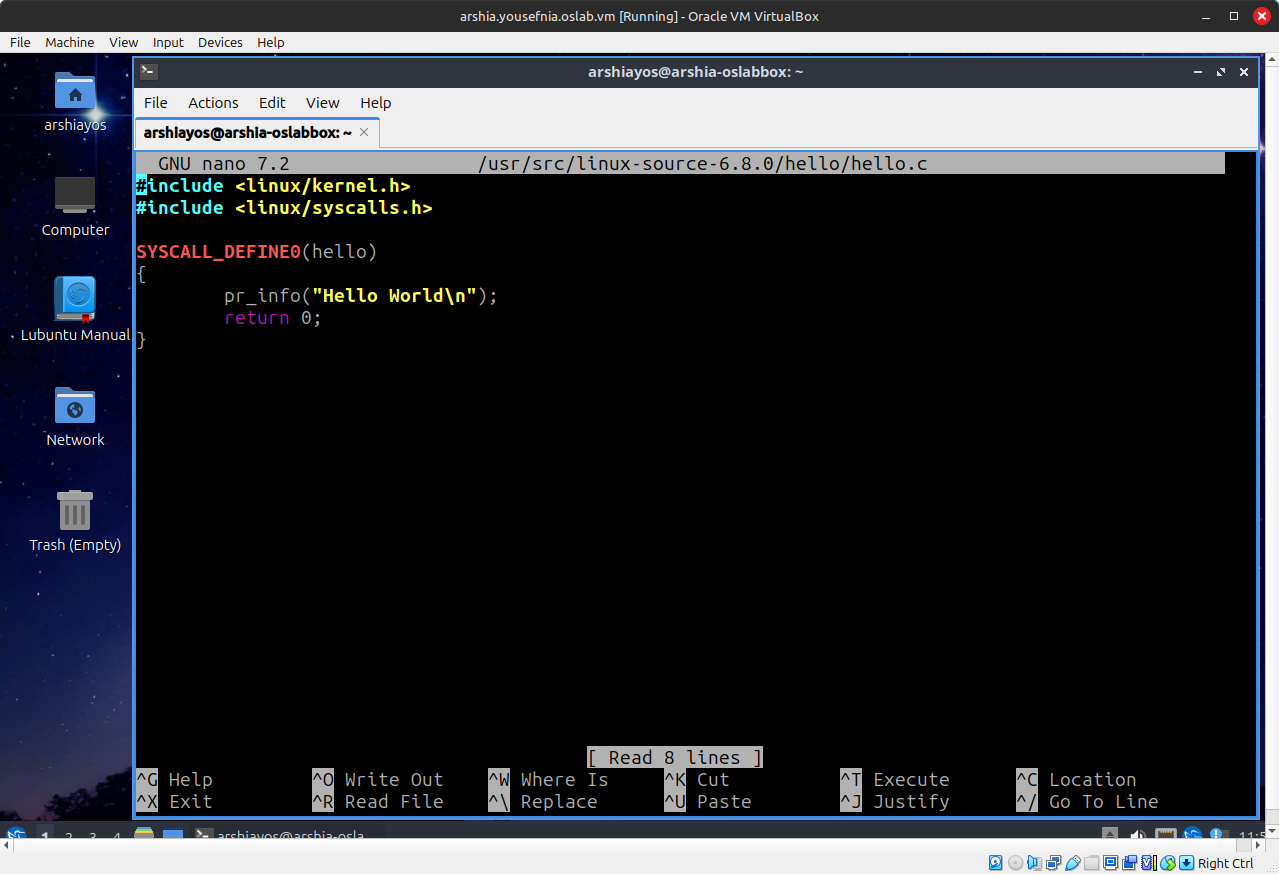
\includegraphics[width=0.8\textwidth]{report2-resources/22-new.png}
		\caption{محتویات فایل \textenglish{hello.c}}
	\end{figure}

        \item 
        \textenglish{Makefile}
        خواسته شده را در پوشه‌ی 
        \textenglish{hello}
        ساخته و محتوای گفته شده را در آن قرار می‌دهیم.

        \begin{figure}[H]
		\centering
		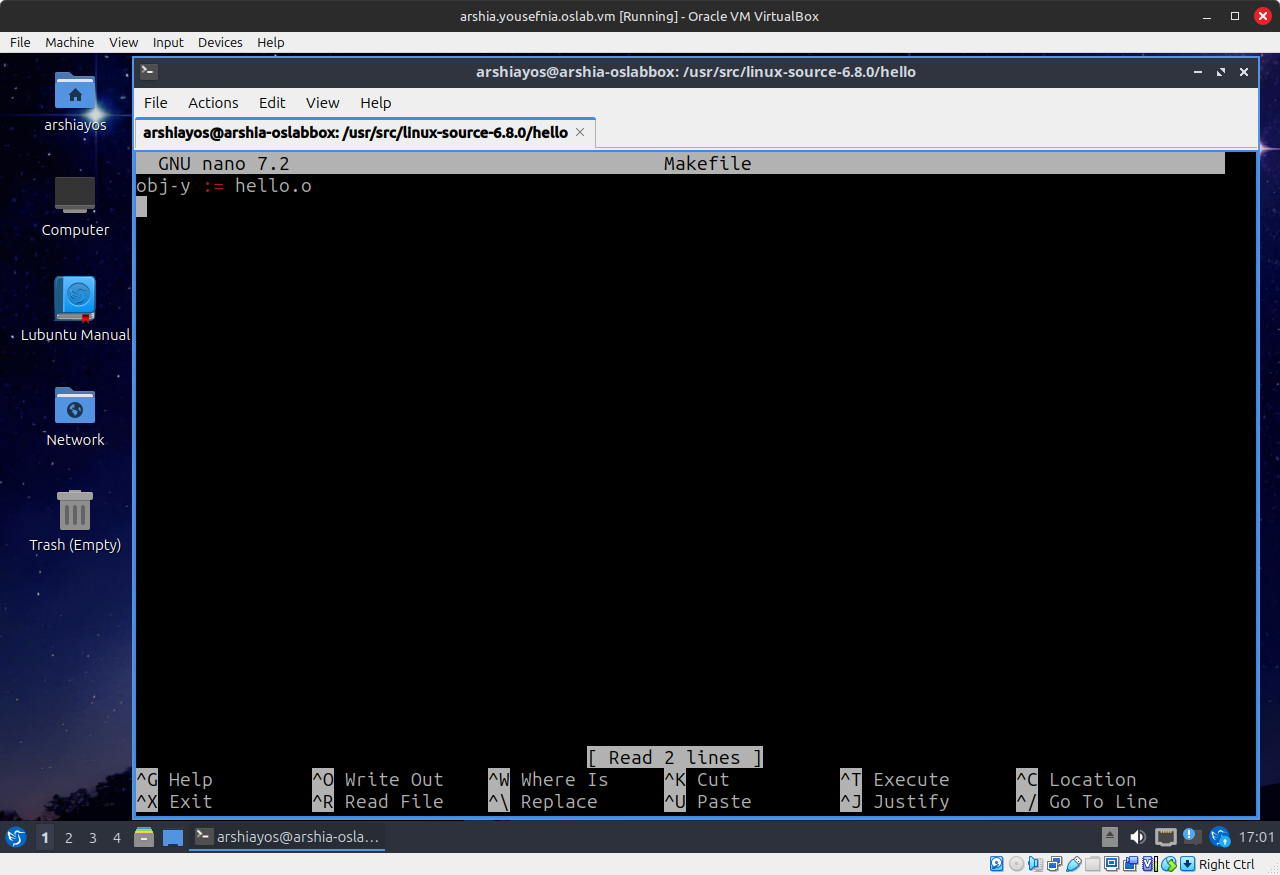
\includegraphics[width=0.8\textwidth]{report2-resources/23.png}
		\caption{محتویات \textenglish{Makefile} موجود در \textenglish{hello}}
	\end{figure}

        \item 
        فایل 
        \textenglish{Kbuild}
        موجود در ریشه‌ی کد منبع را باز کرده و 
        \textenglish{hello/}
        را در مکان خواسته شده به 
        پ
        \textenglish{obj-y}
        اضافه می‌کنیم.

        \begin{figure}[H]
		\centering
		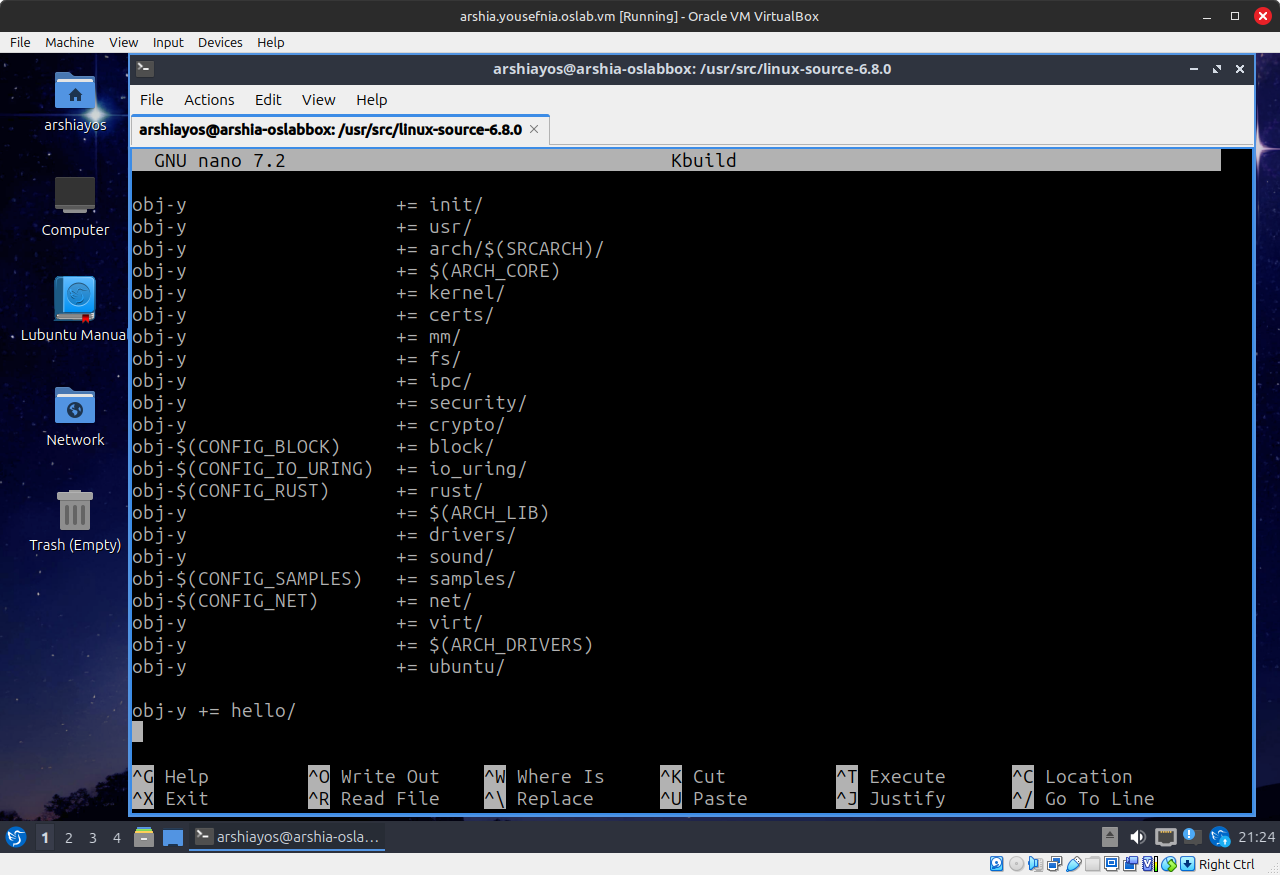
\includegraphics[width=0.8\textwidth]{report2-resources/28.png}
		\caption{محتویات \textenglish{Kbuild} موجود در ریشه‌ی کد منبع}
	\end{figure}

        \item 
        فایل خواسته شده را باز کرده و خطی مشابه خط گفته شده را به آن اضافه می‌کنیم (به دلیل تفاوت در نسخه‌ی سیستم عامل، کمی نام فایل‌ها و خط اضافه شده با چیزی که در دستور کار گفته شده بود تفاوت دارد).

        \begin{figure}[H]
		\centering
		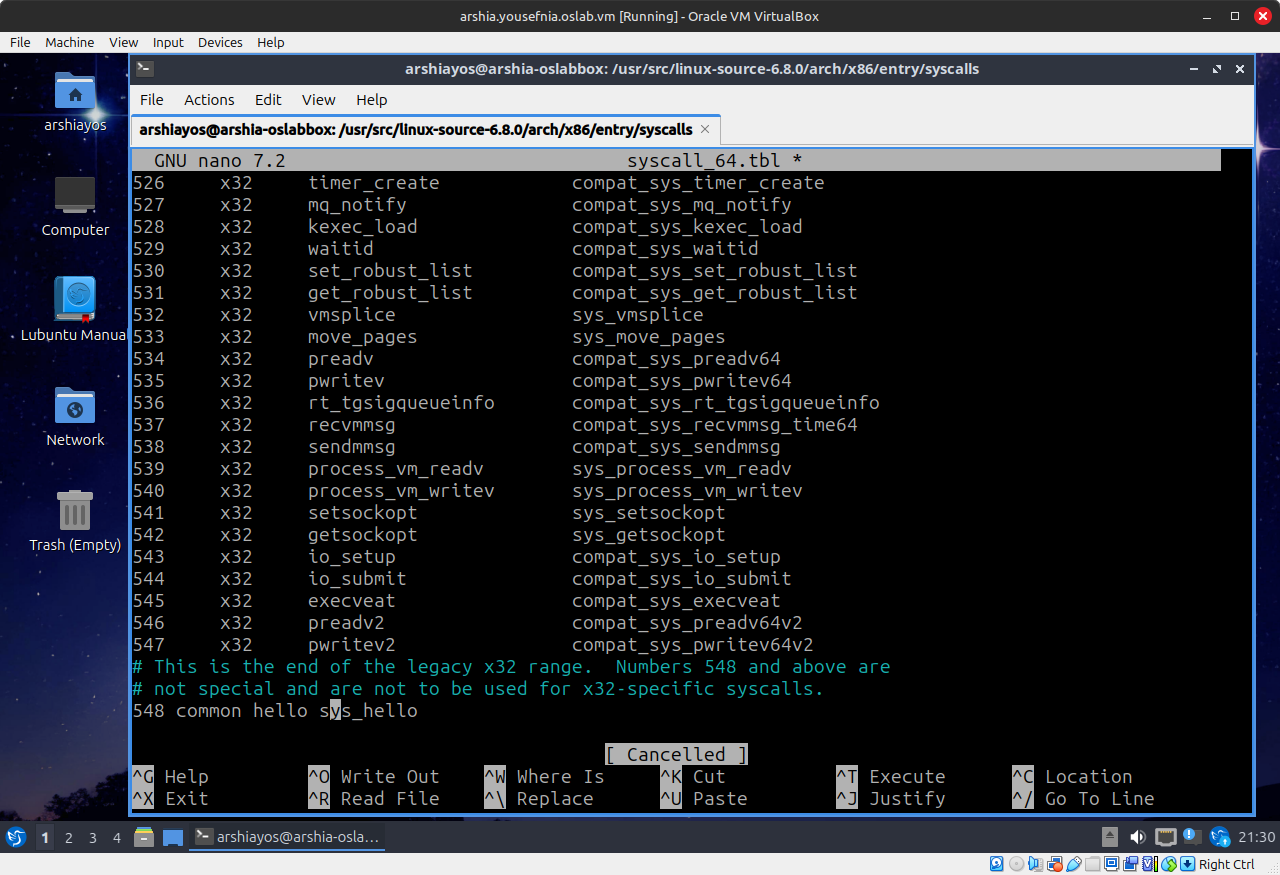
\includegraphics[width=0.8\textwidth]{report2-resources/30.png}
		\caption{اضافه کردن تابع فراخوانی سیستمی ساخته شده به لیست فراخوانی‌های سیستمی}
	\end{figure}

        \item 
        در فایل گفته شده در صورت سوال، خط زیر را اضافه می‌کنیم.

        \begin{figure}[H]
		\centering
		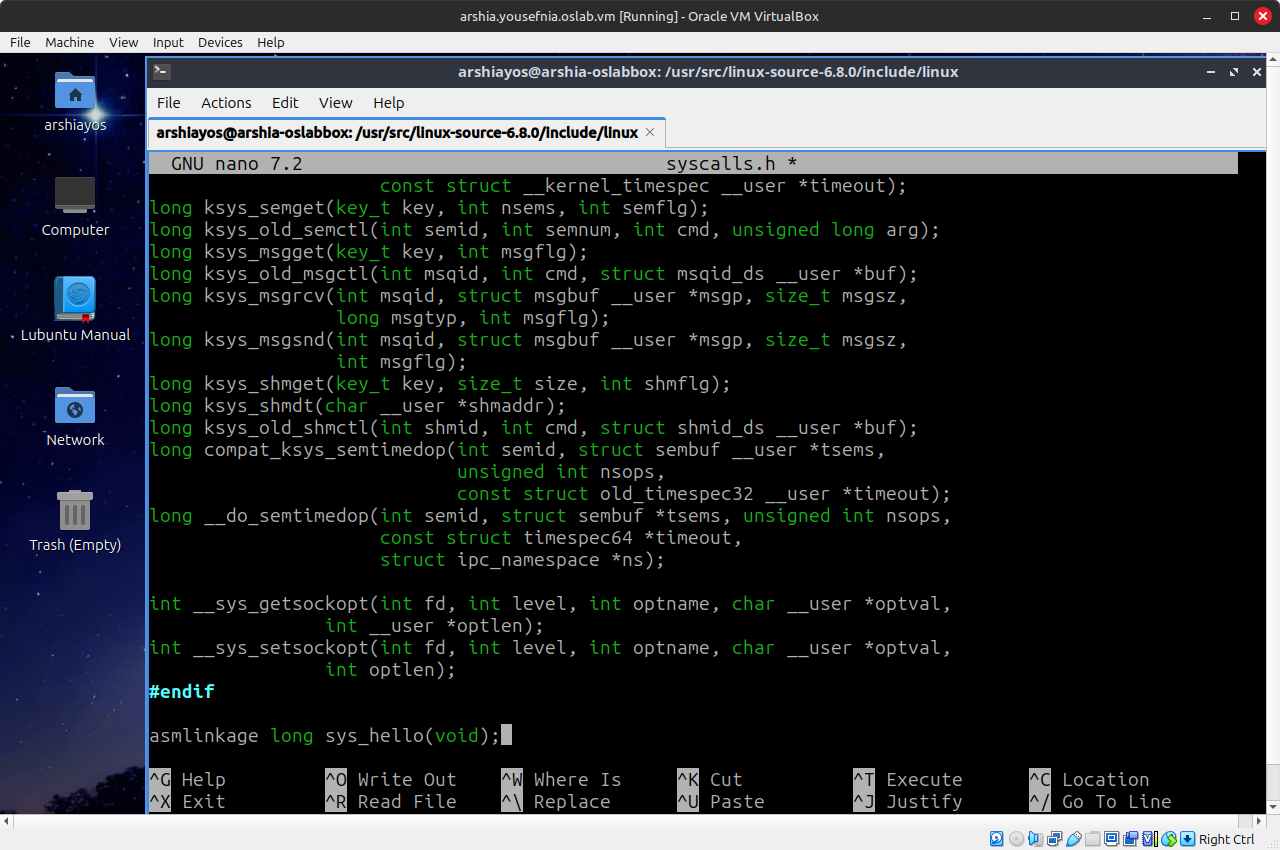
\includegraphics[width=0.8\textwidth]{report2-resources/26.png}
		\caption{خط اضافه شده به فایل \textenglish{syscalls.h}}
	\end{figure}

        \item 
        هسته را مجدد کامپایل کرده و نصب می‌کنیم.

        \begin{figure}[H]
		\centering
		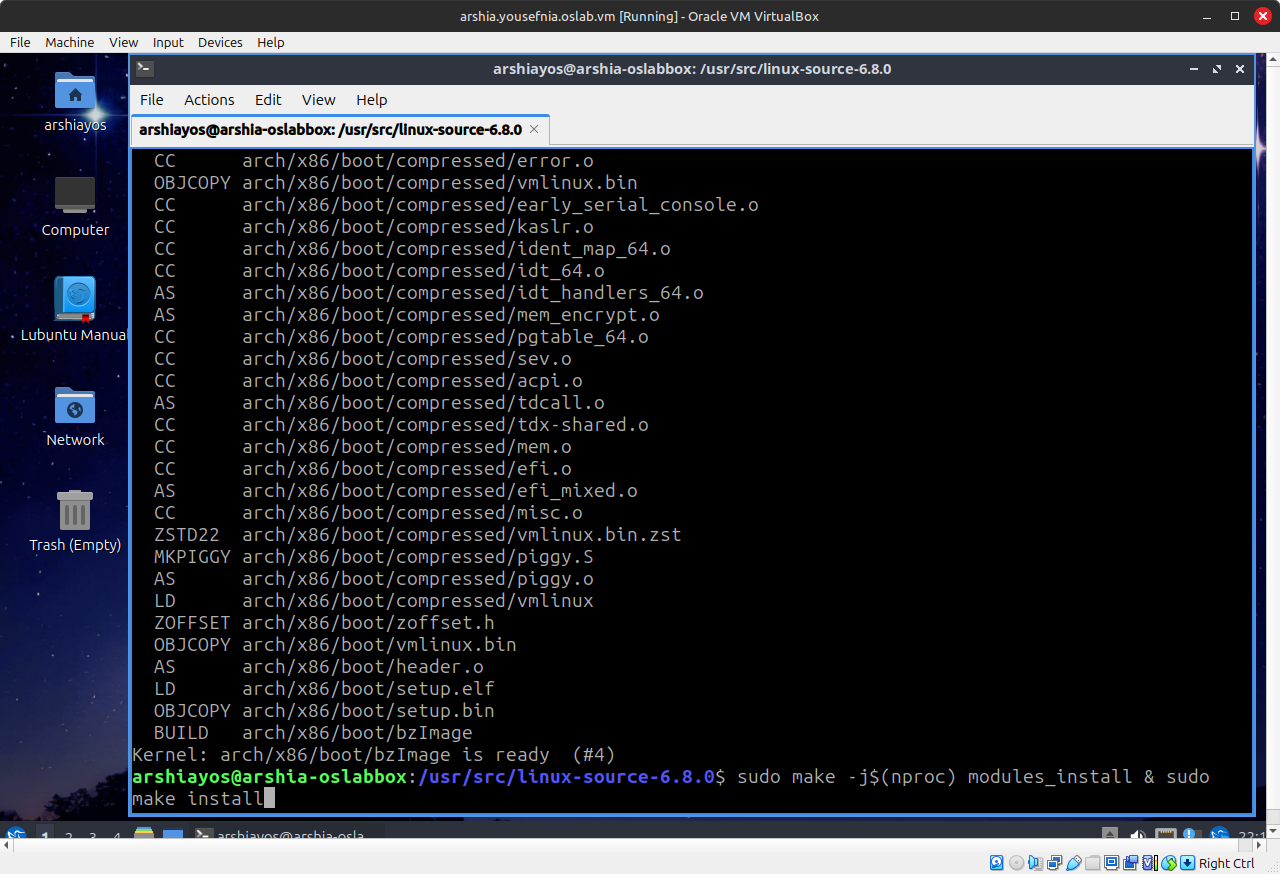
\includegraphics[width=0.8\textwidth]{report2-resources/31.png}
		\caption{کامپایل و نصب مجدد هسته}
	\end{figure}
        
        
        \end{enumerate}
        
        حال که فراخوانی سیستم به سیستم عامل اضافه شد، با 
        \textenglish{reboot}
        کردن سیستم می‌توان از آن فراخوانی سیستمی استفاده کرد.

        حال تمارین این بخش را انجام می‌دهیم.

        \begin{itemize}
        \item ابتدا برنامه‌ای می‌نویسیم که با دستور
        \textenglish{syscall}
        فراخوانی سیستمی اضافه شده را اجرا کند.
        می‌دانیم شماره‌ی این فراخوانی سیستمی 
        \textenglish{548}
        است و آرگومان ورودی ندارد. پس برنامه‌ی خواسته شده به صورت شکل زیر می‌شود:

        \begin{figure}[H]
		\centering
		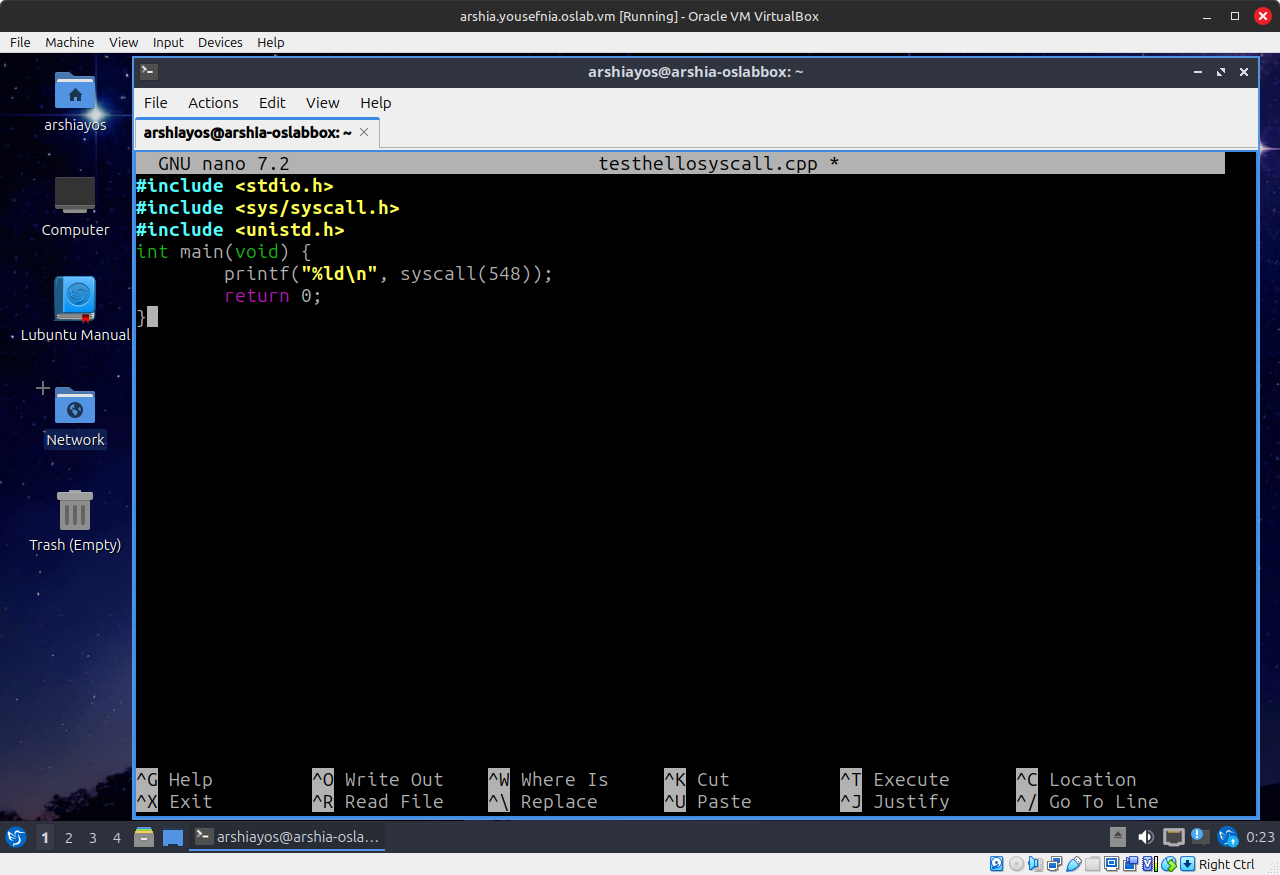
\includegraphics[width=0.8\textwidth]{report2-resources/33.png}
		\caption{استفاده از فراخوانی سیستمی \textenglish{hello} در کد یک برنامه}
	\end{figure}

        سپس این برنامه را کامپایل و اجرا کرده و با دستور 
        \textenglish{dmesg}
        (صرفا چاپ کردن چند خط آخر آن با دستور 
        \textenglish{tail})
        می‌توان دید که فراخوانی‌ سیستمی اجرا شده است.

        \item 
        از آنجایی که قبلا مراحل اضافه کردن فراخوانی سیستمی گفته شده، در بخش‌های تکرار توضیحی نداده و صرفا از مراحل اسکرین شات می‌گذاریم.

        \begin{figure}[H]
		\centering
		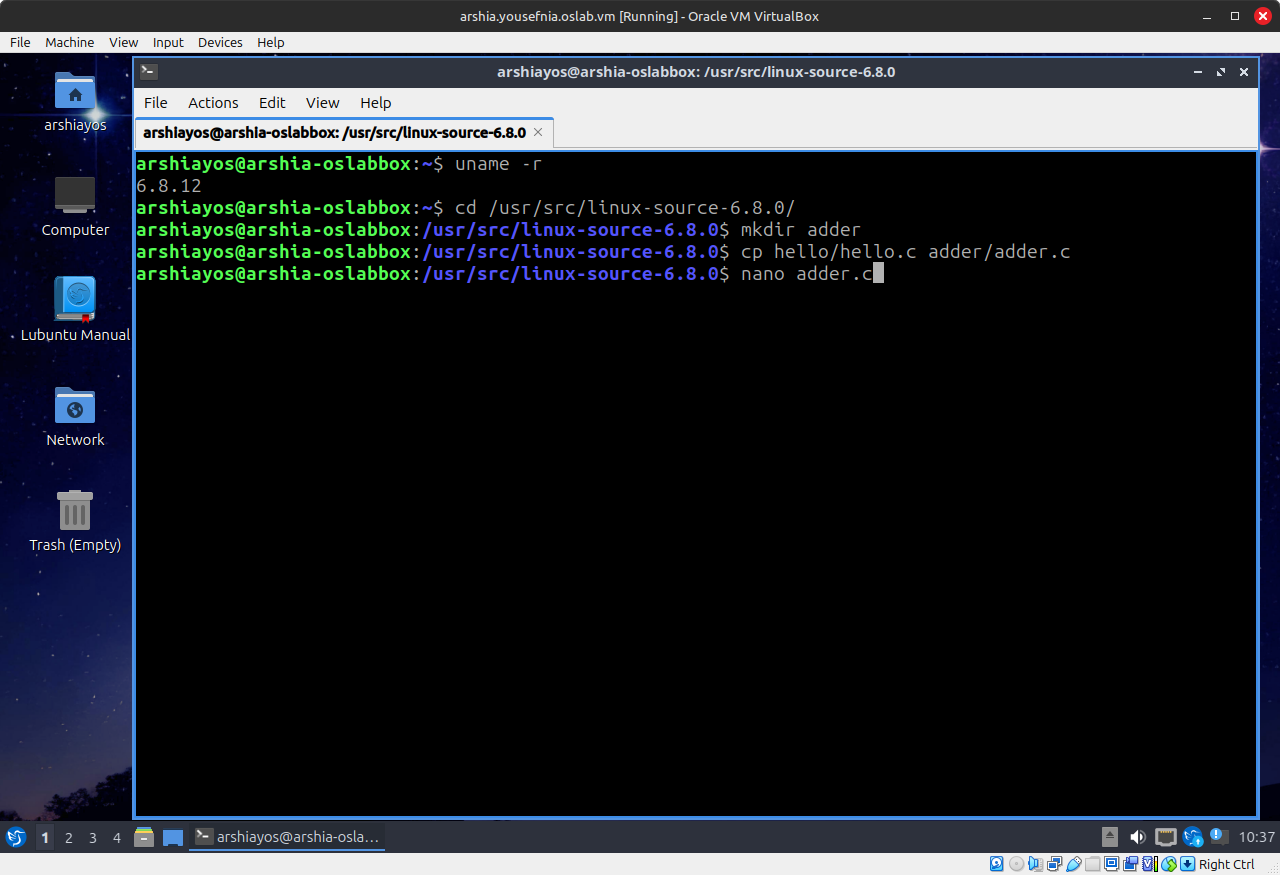
\includegraphics[width=0.8\textwidth]{report2-resources/35.png}
		\caption{اضافه کردن پوشه‌ی \textenglish{adder}}
	\end{figure}

        کد فراخوانی سیستمی، علاوه بر دادن خروجی مناسب، ورودی‌ها و خروجی را چاپ می‌کند تا بررسی آن در آینده راحت‌تر شود.
        
        \begin{figure}[H]
		\centering
		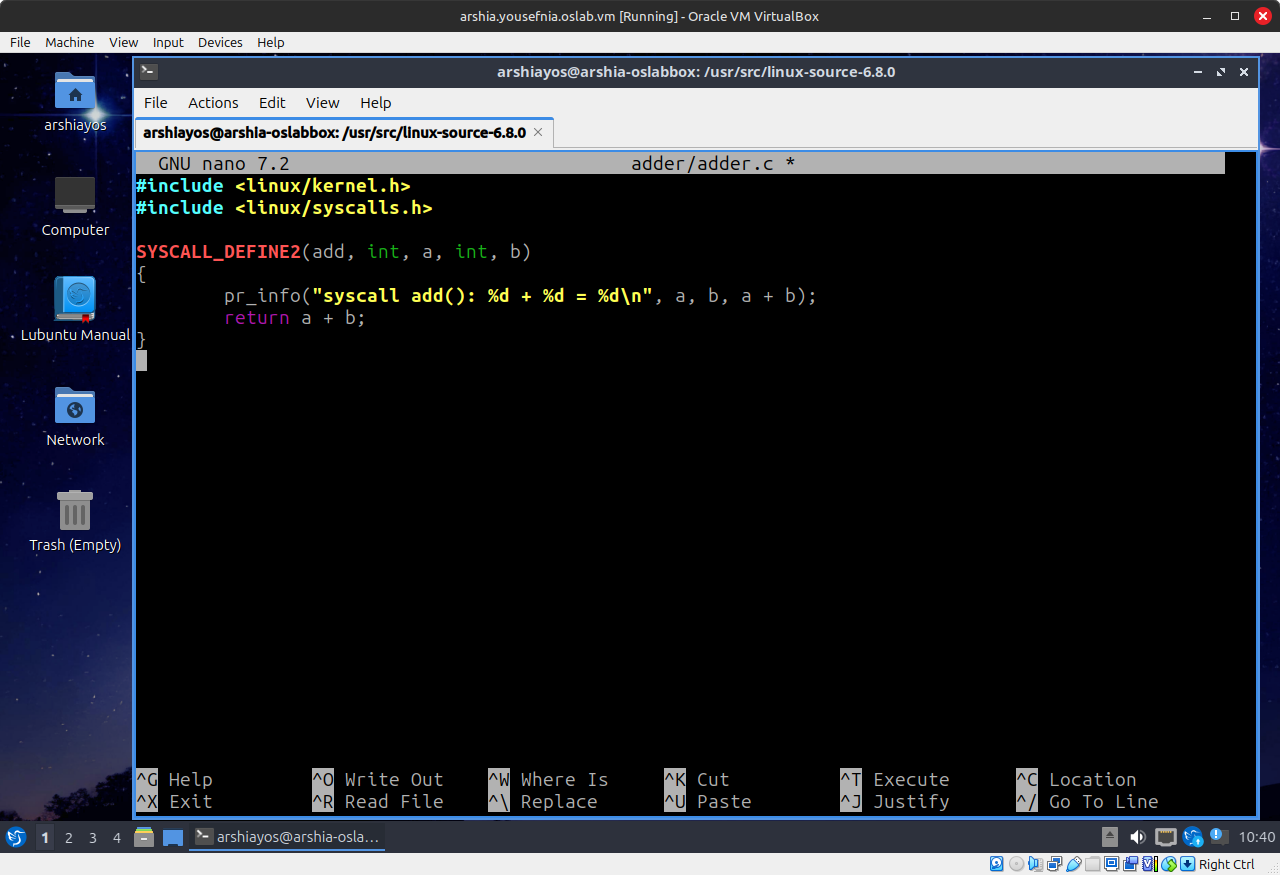
\includegraphics[width=0.8\textwidth]{report2-resources/36.png}
		\caption{کد فراخوانی سیستمی \textenglish{adder}}
	\end{figure}

        \begin{figure}[H]
		\centering
		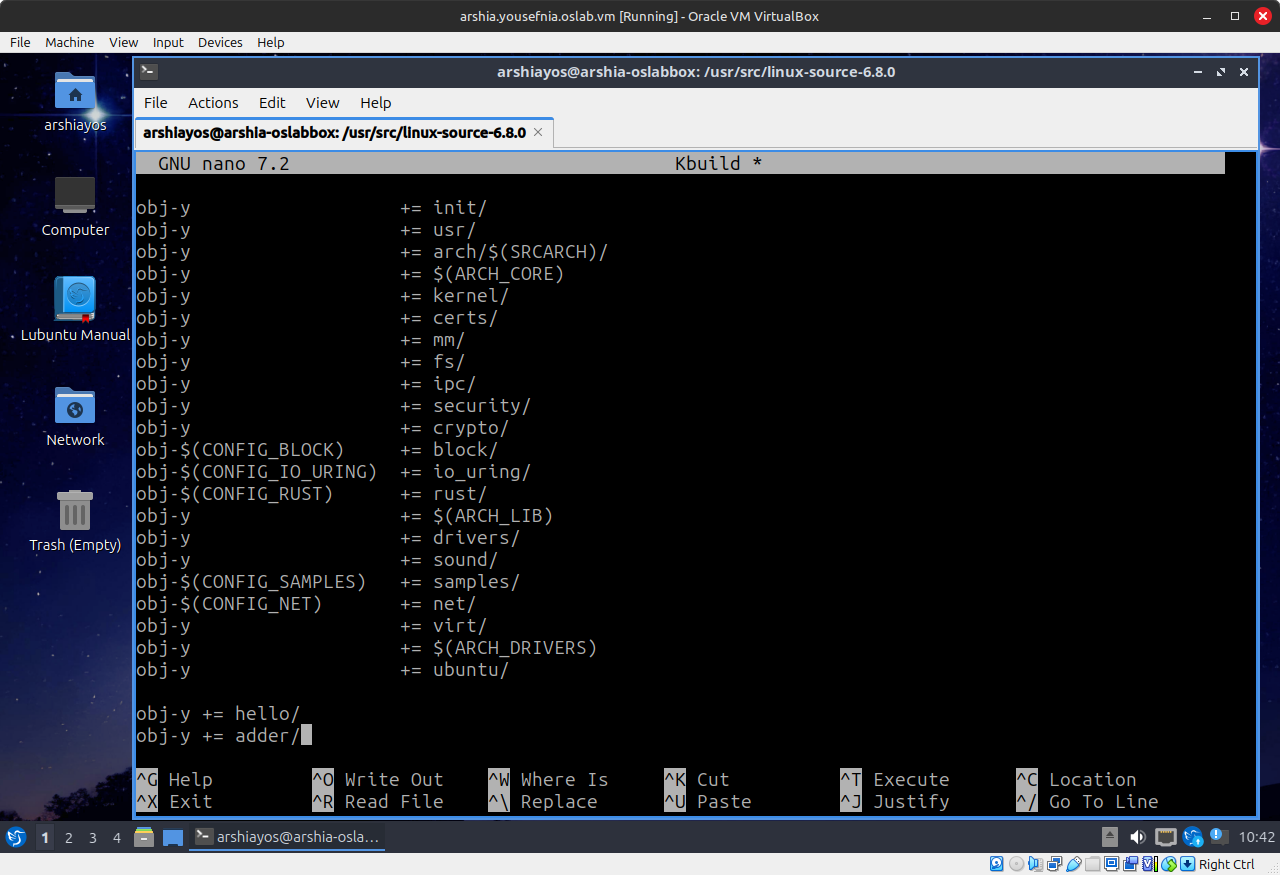
\includegraphics[width=0.8\textwidth]{report2-resources/37.png}
		\caption{اضافه کردن \textenglish{adder} به \textenglish{Kbuild}}
	\end{figure}

        \begin{figure}[H]
		\centering
		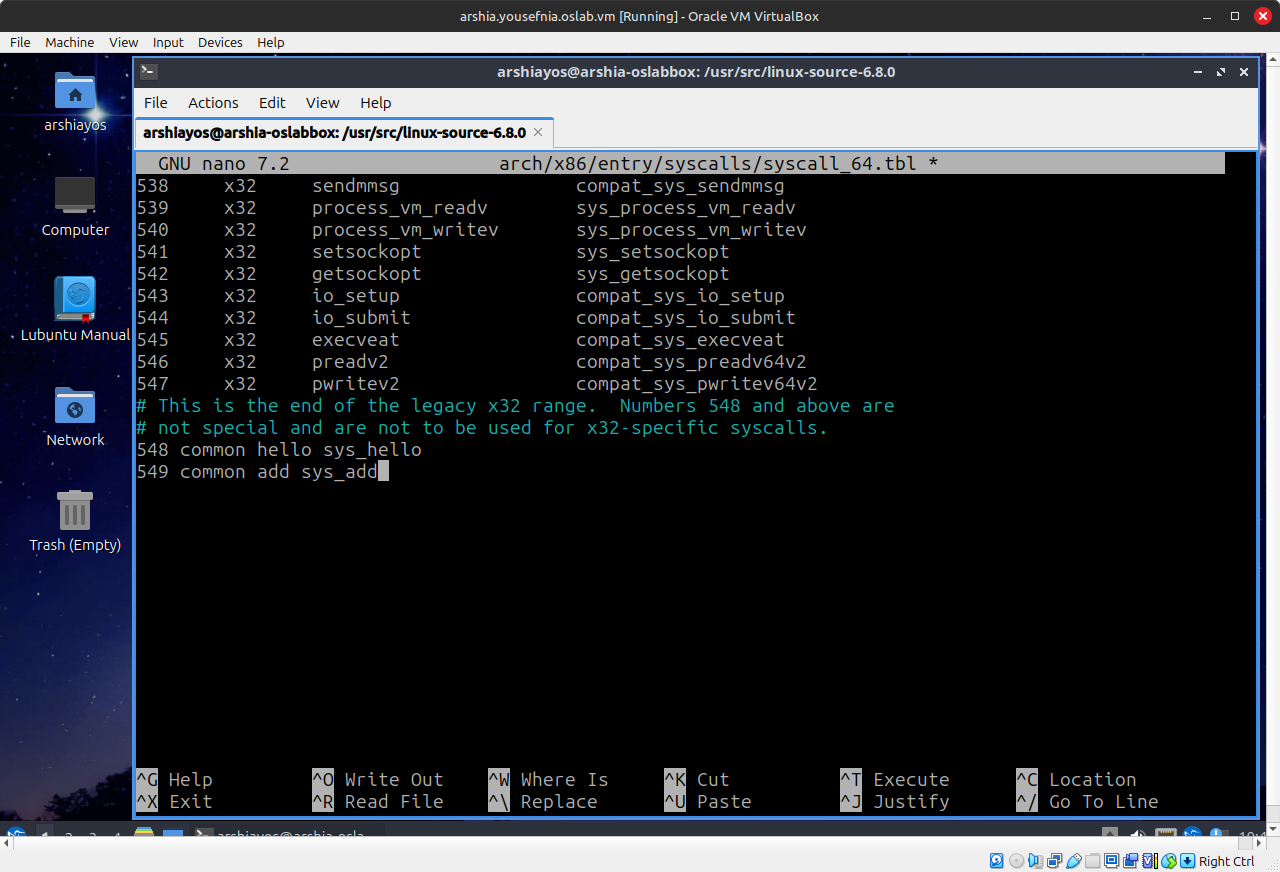
\includegraphics[width=0.8\textwidth]{report2-resources/38.png}
		\caption{اضافه کردن \textenglish{adder} به لیست فراخوانی‌های سیستم}
	\end{figure}

        \begin{figure}[H]
		\centering
		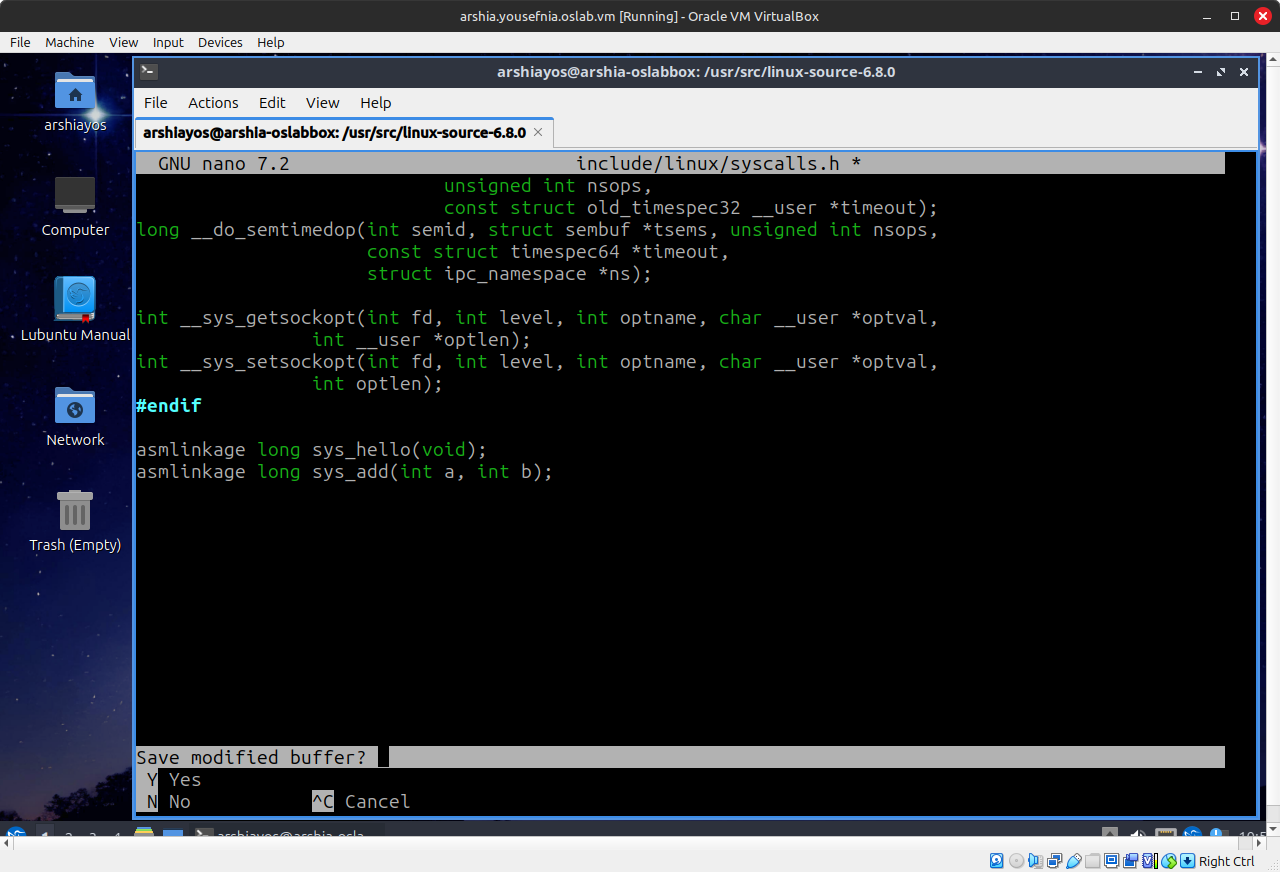
\includegraphics[width=0.8\textwidth]{report2-resources/39.png}
		\caption{اضافه کردن \textenglish{adder} به \textenglish{syscalls.h}}
	\end{figure}

        \begin{figure}[H]
		\centering
		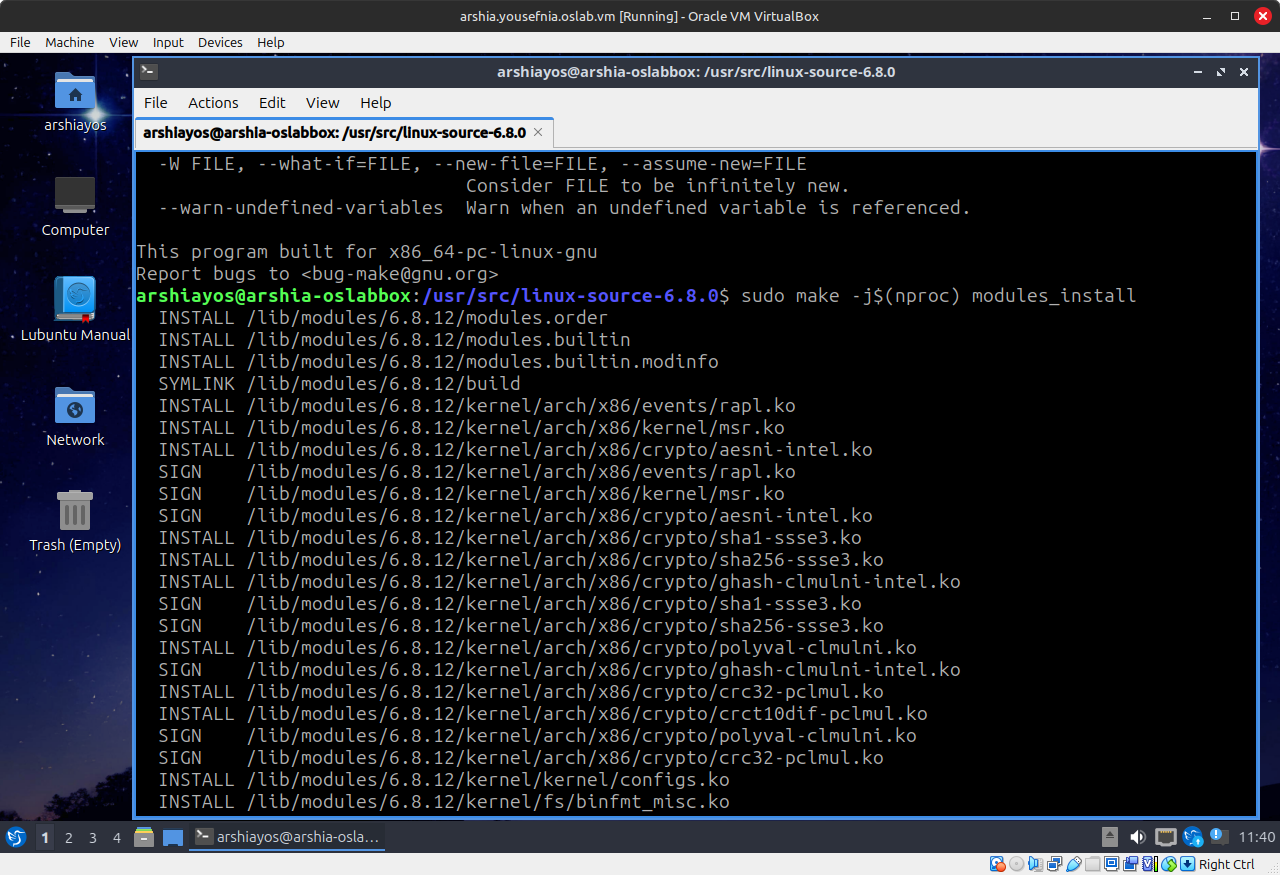
\includegraphics[width=0.8\textwidth]{report2-resources/41.png}
		\caption{کامپایل مجدد هسته و نصب ماژول‌ها}
	\end{figure}

        \begin{figure}[H]
		\centering
		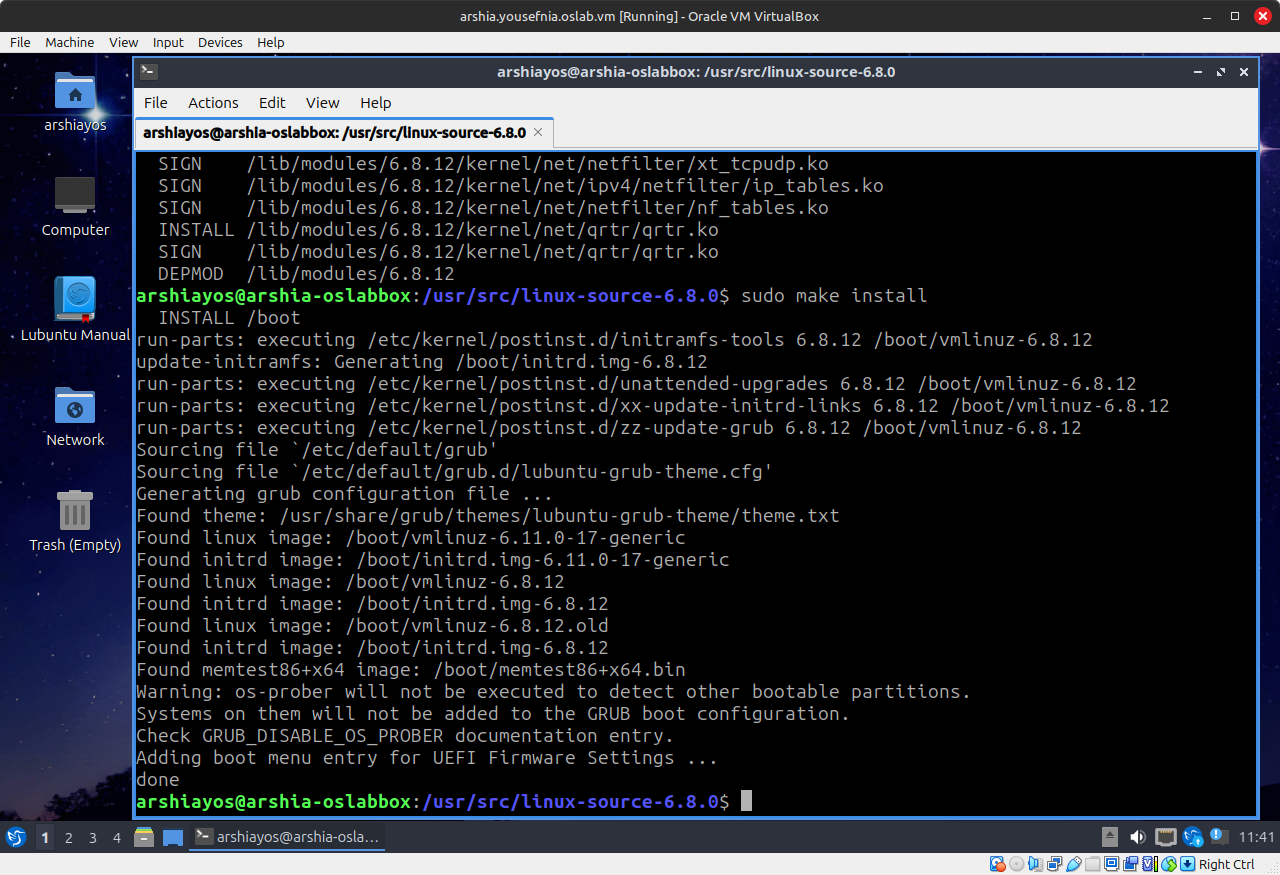
\includegraphics[width=0.8\textwidth]{report2-resources/42.png}
		\caption{نصب مجدد هسته}
	\end{figure}

        \begin{figure}[H]
		\centering
		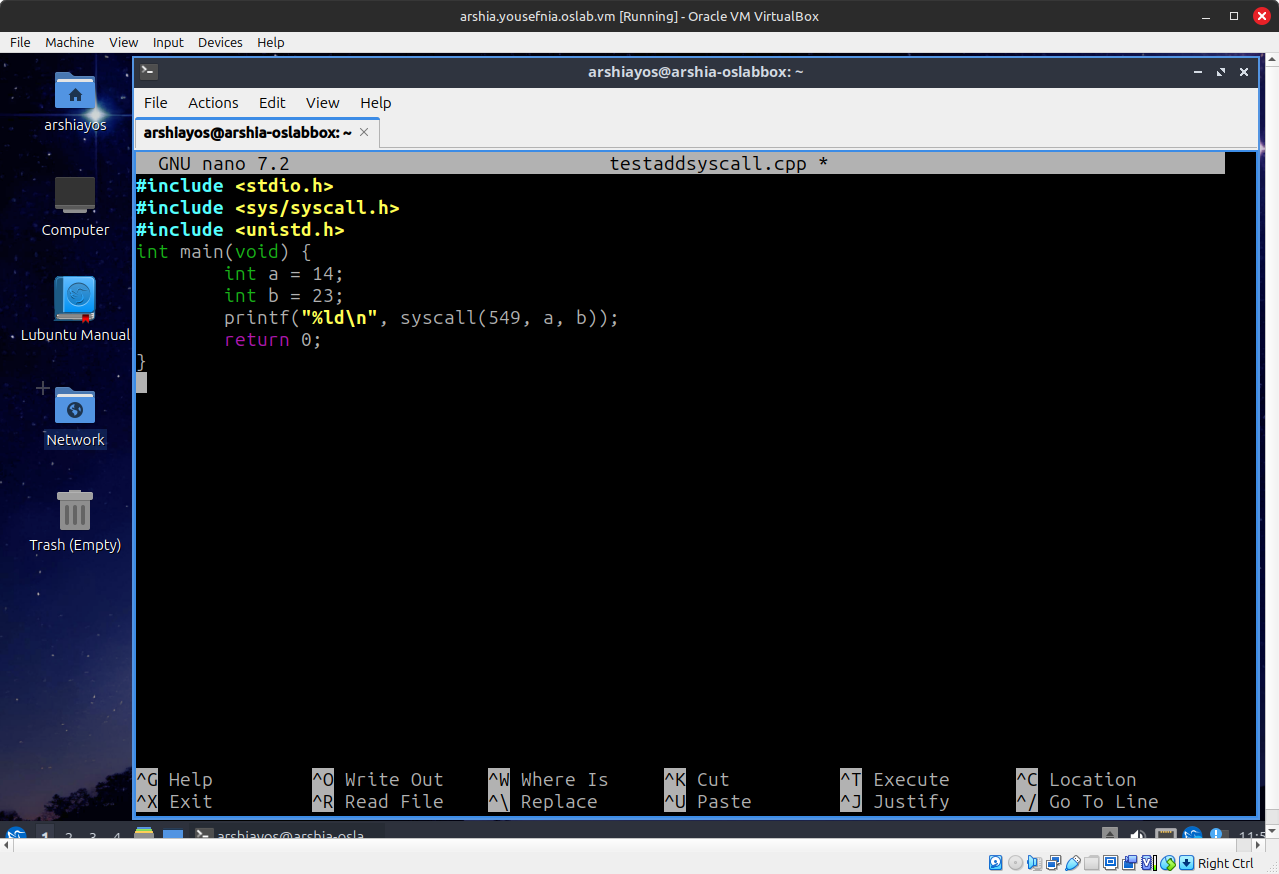
\includegraphics[width=0.8\textwidth]{report2-resources/43.png}
		\caption{نوشتن برنامه‌ای که از فراخوانی سیستمی \textenglish{adder} استفاده می‌کند}
	\end{figure}

        \begin{figure}[H]
		\centering
		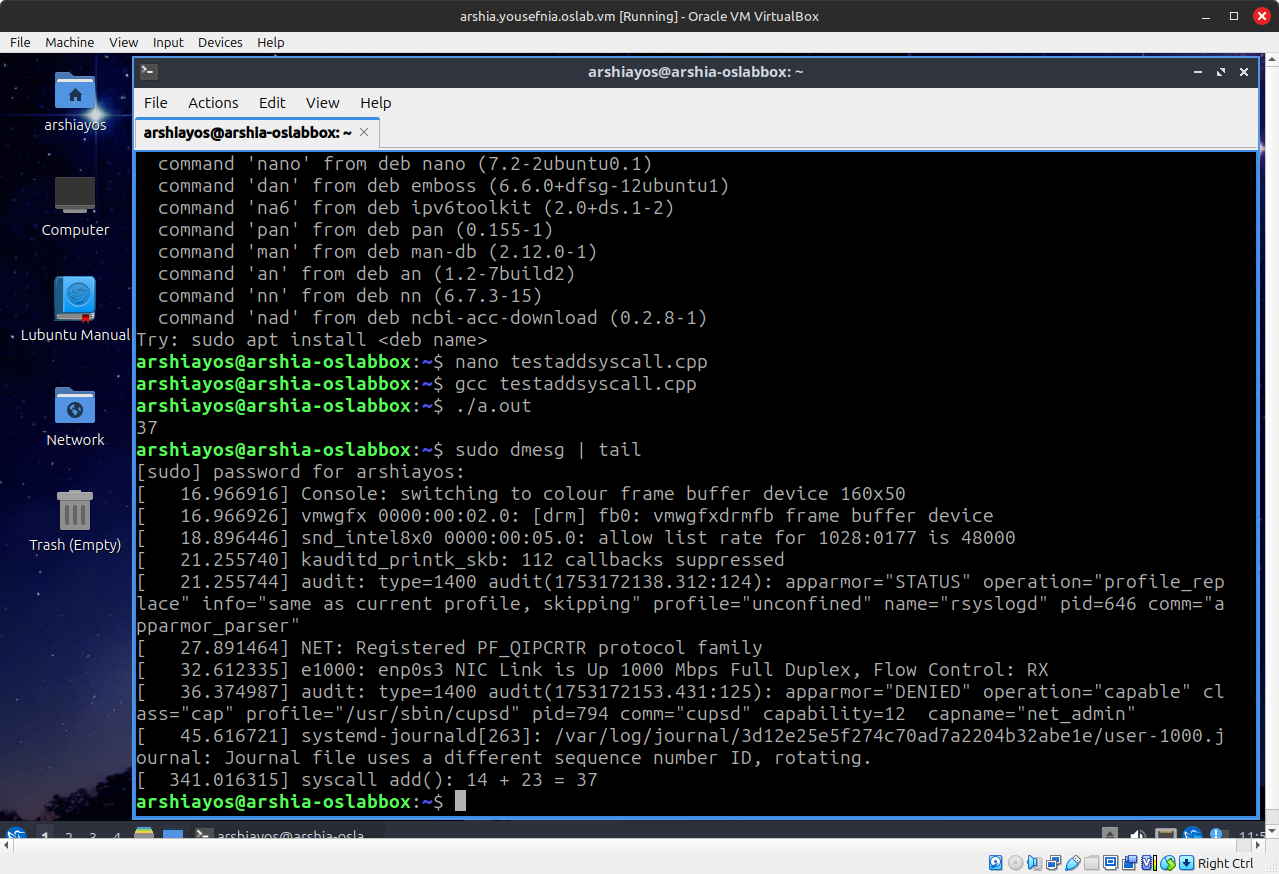
\includegraphics[width=0.8\textwidth]{report2-resources/44.png}
		\caption{خروجی برنامه‌ی بالا}
	\end{figure}
        \end{itemize}
    
	
	% ==============================
	% References
	% ==============================
	\newpage
	\begin{LTR}
		\begin{english}
                \printbibliography[title={مراجع}]
            \end{english}
	\end{LTR}

	
\end{document}

